%%%%%%%%%%%%%%%%%%%%
% Introduction chapter

%%%%%%%%%%%%%%%%%%%%%%%%%%%%%%%%%%%%%%%%
%%%%%%%%%%%%%%%%%%%%%%%%%%%%%%%%%%%%%%%%
% \section{Hypothesis and goals}
%%%%%%%%%%%%%%%%%%%%%%%%%%%%%%%%%%%%%%%%
%%%%%%%%%%%%%%%%%%%%%%%%%%%%%%%%%%%%%%%%

%%%%%%%%%%%%%%%%%%%%%%%%%%%%%%%%%%%%%%%%
Meiosis occurs in all sexually reproducing organisms, and is essential to gametogenesis.
Recombination plays a key role in this process, facilitating the pairing and alignment of chromosomes, while the exchange of genetic material has important implications in inheritance, natural selection, and evolution.
Double strand breaks begin the recombination process, and resolve to one of two outcomes, crossover or gene conversion (outlined in Figure \ref{fig:introOutcomes}).
% Crossover is the reciprocal exchange of genetic material around the break point, while gene conversion is the uni-directional transfer of small amounts segments of DNA from one chromosome to its homologue.
Most research  has focused on genetic crossover, which is the reciprocal exchange of genetic material between homologous chromosomes during meiosis.

There are a number of factors that influence the placement of crossovers within the genome, and there is tremendous variability between individuals, sexes, and species.
Recombination properties differ greatly between males and females, both in frequency and in placement within the genome.
% In addition, recombination in most mammals has been shown to be preferentially located into hotspots, narrow regions within the genome.
% Hotspots are under the control of the PRDM9 protein, and much research has focused on their further characterization.
%
In this introductory chapter, I will review historical literature that has advanced our understanding of recombination, building up to the current knowledge of how recombination is affected by these recombination modifying factors.
Much of existing research focuses on human subjects, and I have focused the majority of work within this thesis on the research of recombination in humans, with the specific goal of learning more about human recombination.
I have focused on research in humans, but consider recombination across a number of other species as well.

% I will review the current and historical literature that has advanced our understanding of how recombination varies in its frequency and placement within the genome.
%Biology / molecular
First, I will review what is known about the biology of meiotic recombination.
This includes the cellular stages that make up meiosis I and II, and how double strand breaks are initiated and resolved. % to either crossover or gene conversion.
%Methods: ld/pedigree
Then I will outline a variety of methods that have been used to study recombination.
This includes molecular methods that observe recombination in a direct fashion, as well as indirect approaches that rely on inferring crossover from genetic data from families and unrelated individuals.
%History / Maps

I will then describe what is currently known about the various factors that act together to modify properites of recombination freqeuncy and placement.
% PRDM9
This includes the hotspot specifying protein PRDM9, which was recently identified, and influences recombination placement in humans and other mammals.
%Sex differences
Another important modifier of recombination is sex, and males and females have been shown to vary widely in their recombination properties on both broad and fine scales.
% Interference
In addition, a phenomenon called interference affects the spacing of bewteen crossover events on a chromosome.

\afterpage{
\begin{figure}[P]
    \begin{center}
    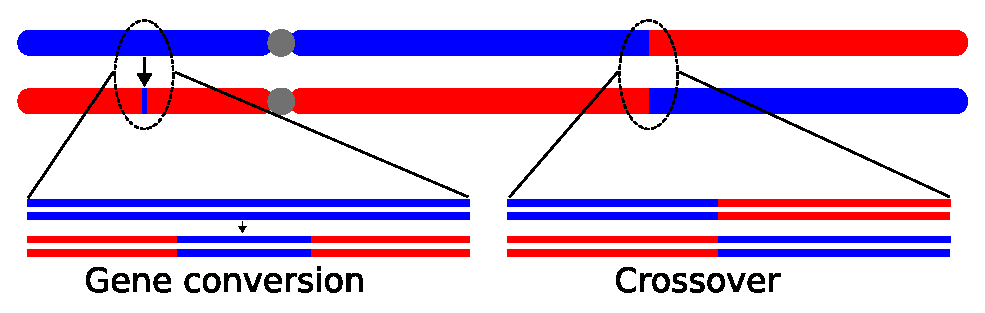
\includegraphics[width=\textwidth]{introduction/figs/outcome_CO-GC}
    \end{center}
    \vspace{-10pt}
    \captionTitle{\textbf{Recombination produces crossover and gene conversion.}}{ 
        Recombination is initiated by DNA double strand breaks that resolve into one of two possible outcomes.
        Crossover (shown at right) is the large-scale, reciprocal exchange of genetic material between two chromosomes around the break point.
        Gene conversion (or non-crossover, shown at left) is the one-way transfer of small amounts of DNA from one chromosome to the other during the repair of the break.
   \label{fig:introOutcomes}}
\end{figure}
\clearpage}

Gene conversion, the non-reciprocal transfer of genetic material between chromosomes is understudied due to the difficulty of its detection.
Most research so far has relied on sperm typing, which does not provide any information on gene conversion in females.
I will review these, as well as genome wide methods that focus on statistical approaches to infer gene conversion events in genetic data.

%Approach
In this thesis, I used a number of biological and statistical methods to gain insight into factors affecting crossover placement, and into the recombination process as a whole.
I will conclude this introduction with an overview of these methods used to study both crossover and gene conversion.
Specifically, this focuses on obtaining genotypes from family pedigrees followed by a hidden Markov model (HMM) approach to call crossovers.
For gene conversions, I will review several previous HMMs that were used to call recombination in population genetic data.

Overall, the study of recombination has advanced greatly over the past 100 years, with substantial progress made in humans following the completion of the Human Genome Project.
Although a number of advances have been made in recent years, our current understanding of the recombination process is incomplete.
The research presented within this thesis provides an expanded picture of the recombination landscape as a whole.



%%%%%%%%%%%%%%%%%%%%%%%%%%%%%%%%%%%%%%%%%%%%%%%%%%%%%%%%%%%%%%%%%%%%%%%%%%%%%%%%
%%%%%%%%%%%%%%%%%%%%%%%%%%%%%%%%%%%%%%%%%%%%%%%%%%%%%%%%%%%%%%%%%%%%%%%%%%%%%%%%
%%%%%%%%%%%%%%%%%%%%%%%%%%%%%%%%%%%%%%%%%%%%%%%%%%%%%%%%%%%%%%%%%%%%%%%%%%%%%%%%


% In Chapter \ref{ch:cointEsc}, I used a large set of human families to identify crossovers within the genome.
% I used this data to investigate specific properties of recombination frequency and placement and how these properties differ between sexes, individuals, and populations.
% I examined hotspot usage on an individual level, as well as how it differs between males and females, and looked for age effects on recombination within this dataset.
% I also determined how crossover interference varies between individuals, and sexes.
% 
% In Chapter \ref{ch:cointExtras}, I present unpublished data that consists of an extension to Chapter \ref{ch:cointEsc}, which includes the analysis of age effects in humans.
% Additionally, I include a re-analysis of public data from single cell sperm and oocytes.
% Here, I focused on crossover interference properties, which can provide valuable information on how crossover placement varies on an individual level.
% 
% In Chapter \ref{ch:dogPed}, I focused on crossover patterns using a complex pedigree of inbred domestic dogs.
% Dogs, and the entire canid family, are unique among mammals because they have acquired a series of disruptive mutations within its PRDM9 ortholog, rendering this gene inactive in meiosis.
% Since this protein is essential to meiosis in some mammals, its absence raises a number of questions as to how recombination has been altered as a result.
% % Dogs provide an interesting cohort on which to study the effects of the loss of PRDM9 on the recombination landscape as a whole.
% Comparing recombination properties in dogs to those of humans will provide additional insight into recombination in other organisms, and within our own species.
% With this goal in mind, I examine aspects of crossover placement within the genome, including crossover interference, and compare these to human data.
% % This data provides valuable insight into the effects of PRDM9, which is missing in dogs, on crossover within our own species.
% % I have also included a chapter in which I analyse recombination in domestic dogs.
% 
% 
% In Chapter \ref{ch:geneConv}, I focus on gene conversion, an alternate outcome of recombination, in which small segments of DNA are transferred in one direction from one chromosome to its homologue.
% Gene conversion (or non-crossover) is the non-reciprocal transfer of genetic information that is limited to smaller intervals.
% I examined current methods for crossover and gene conversion detection, and based on this I propose a new model to detect gene conversion events using admixed population genetic data.
% 
% In general, this thesis can be divided into two main sections, each focusing on one of the two outcomes of recombination: crossover and gene conversion.
% In part one (Chapters \ref{ch:cointEsc}, \ref{ch:cointExtras}, and \ref{ch:dogPed}), I focus on crossover, using a pedigree approach to study recombination in humans and dogs.
% Part two (Chapter \ref{ch:geneConv}) focuses on a statistical model for the detection of gene conversion events.
% % Overall, 
% These two aspects come together to provide an expanded picture of the recombination landscape as a whole.
% 
% 



%%%%%%%%%%%%%%%%%%%%%%%%%%%%%%%%%%%%%%%%
%%%%%%%%%%%%%%%%%%%%%%%%%%%%%%%%%%%%%%%%
\section{An overview of meiotic recombination}
%%%%%%%%%%%%%%%%%%%%%%%%%%%%%%%%%%%%%%%%
%%%%%%%%%%%%%%%%%%%%%%%%%%%%%%%%%%%%%%%%

\afterpage{
\begin{figure}[P]
    \begin{center}
    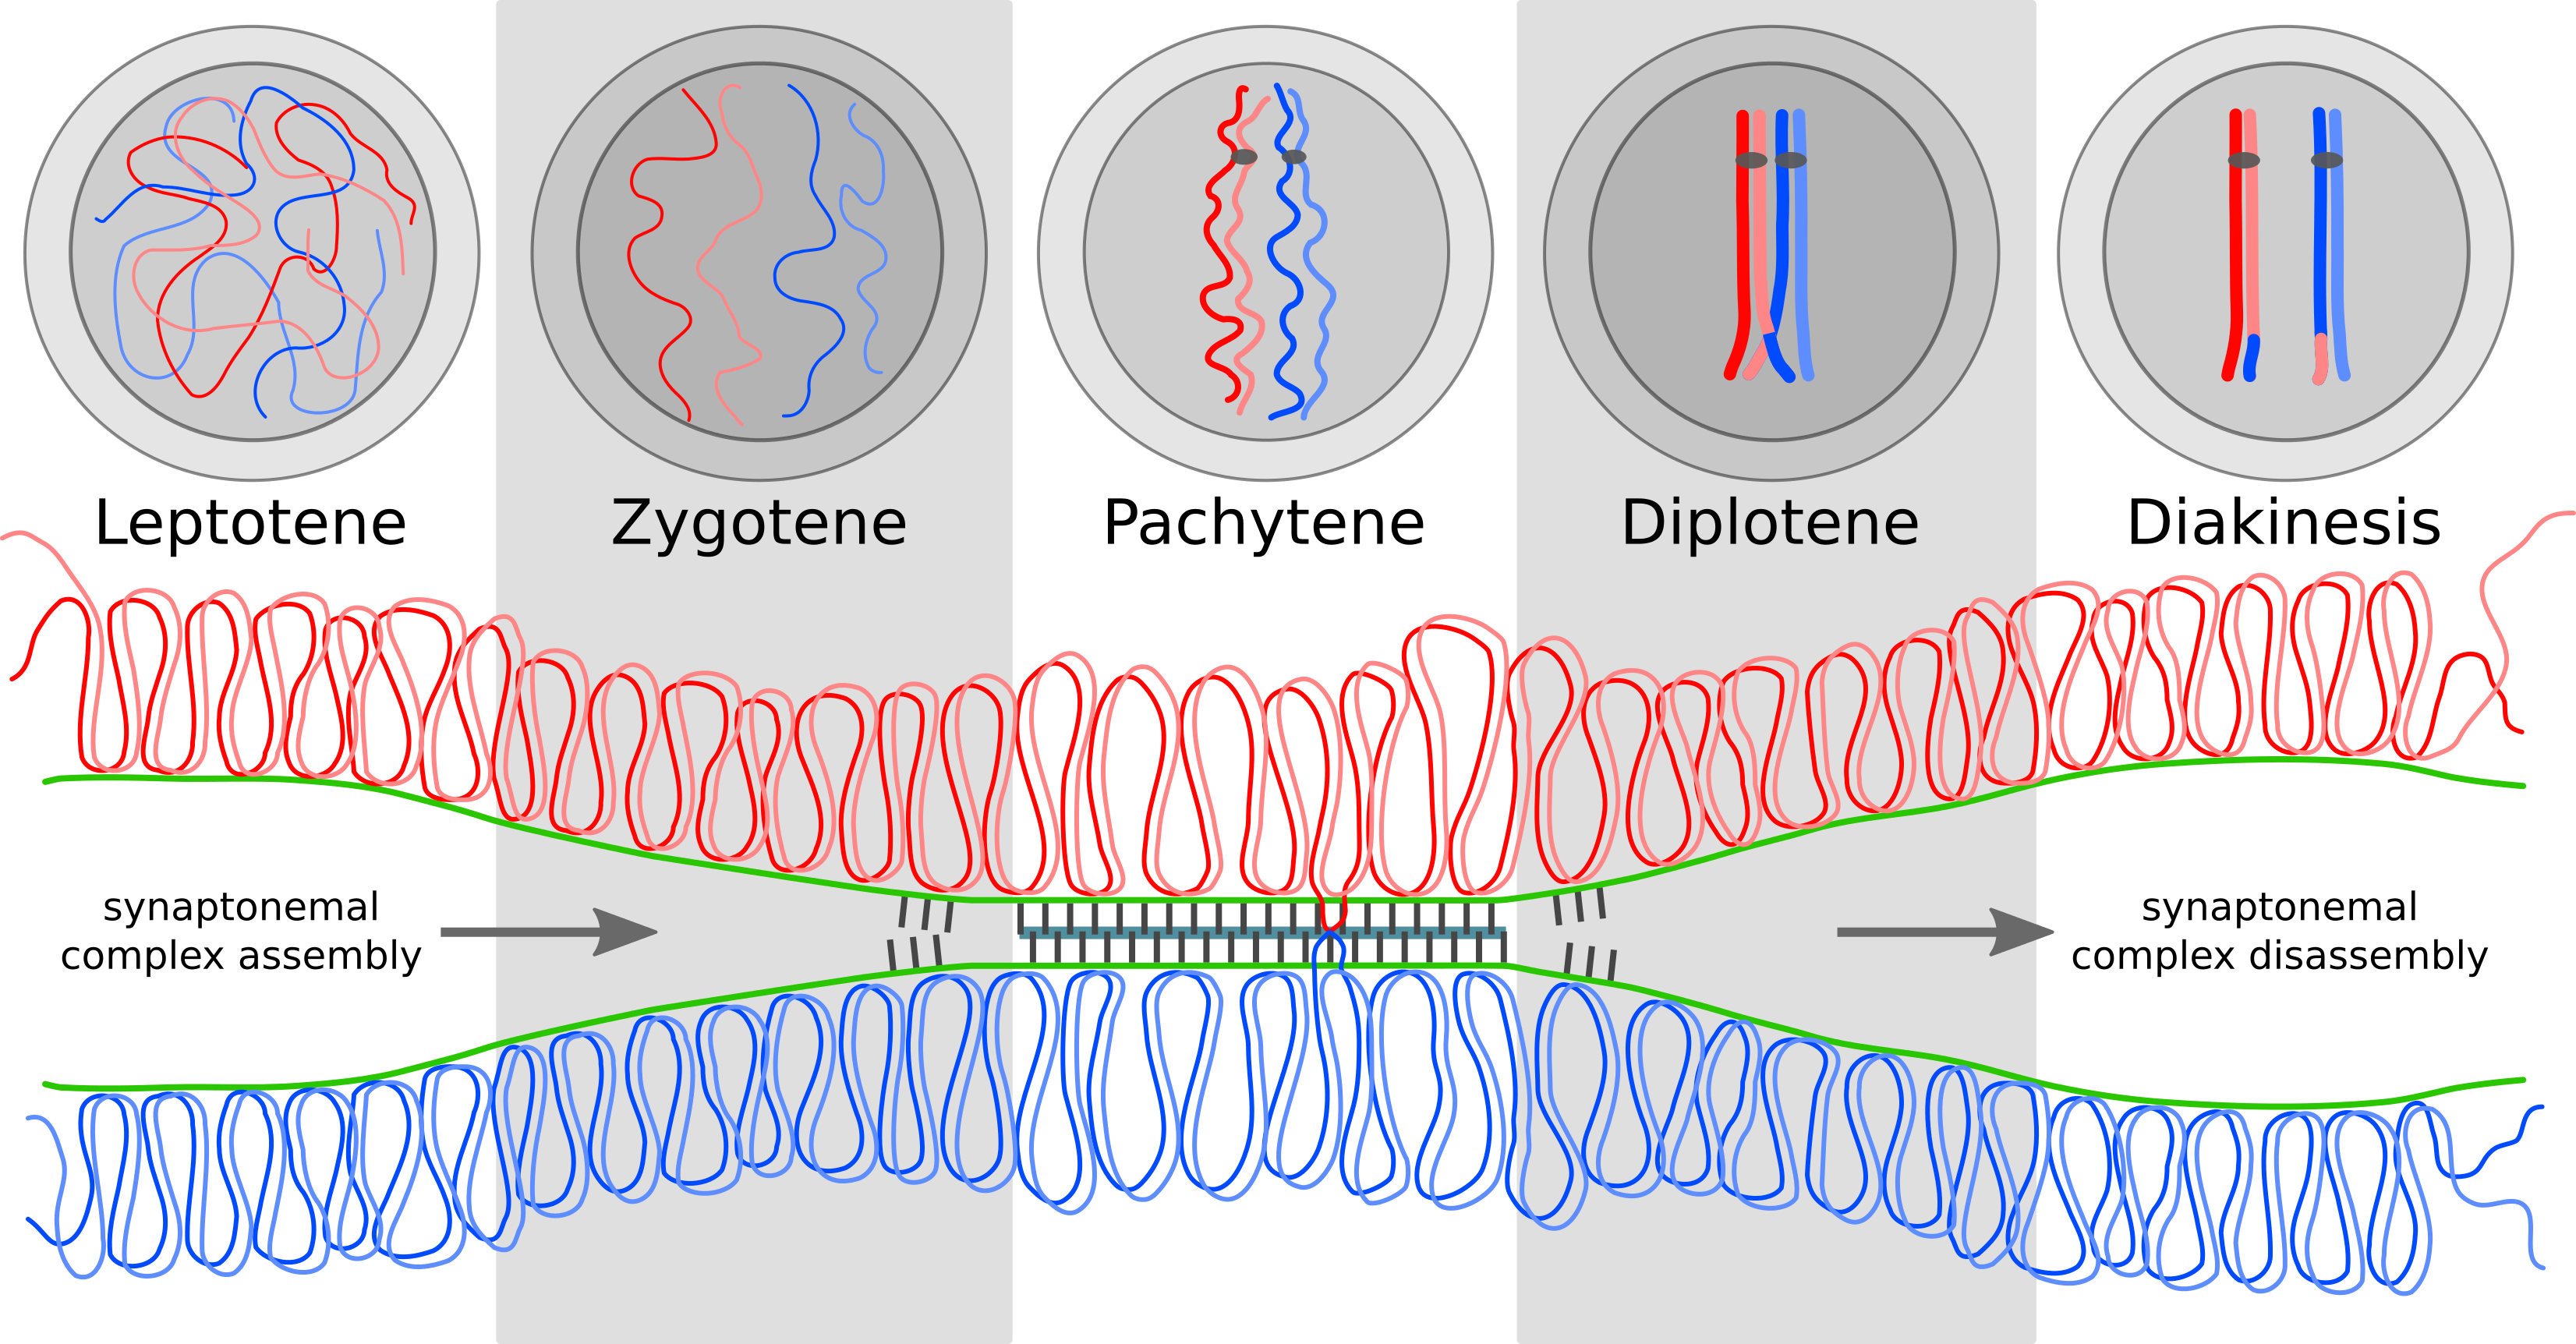
\includegraphics[width=\textwidth]{introduction/figs/prophaseI.png}
    \end{center}
    \vspace{-10pt}
    \captionTitle{\textbf{The stages of prophase I in meiosis.}}{ 
        The top panel shows an overview of the five stages of prophase I, progressing from left to right.
        One pair of sister chromatids is shown in shades of red, and represents genetic material inherited from one parent.
        A second pair of sister chromatids, inherited from the other parent, is shown in shades of blue.
        %and is homologous to the second pair of sister chromatids, shown in shades of blue.
        The pairs of sister chromatids are homologous to each other and this homology aids in pairing and synapsis.
        The bottom panel shows the progression of the assembly and disassembly of the synaptonemal complex (SC), corresponding with the stages in the top panel.
        A recombination event is shown in the pachytene stage, mediated within the central region of the SC.
        The axial element forms the backbone of the SC (shown in green) and binds to DNA that is tightly packaged into large chromatin loops.
        Modified from \citet{Yang2009} and \citet{DeBoer2006}.
   \label{fig:introProphaseI}}
\end{figure}
\clearpage}



%%%%%%%%%%%%%%%%%%%%%%%%%%%%%%%%%%%%%%%%
\subsection{The biology of meiotic recombination}
%%%%%%%%%%%%%%%%%%%%%%%%%%%%%%%%%%%%%%%%

Prior to meiosis, a diploid cell contains pairs of homologous chromosomes, with one of the pair inherited from the father, and the other from the mother.
This diploid DNA is replicated just prior to the cell entering the meiotic cycle, in premeiotic S-phase\cite{Bell2002} to generate exact copies of each pair of chromosomes, referred to as sister chromatids.
Meiosis consists of two stages; recombination occurs in the first stage, referred to as meiosis I, while sister chromatids separate into their respective daughter cells in meiosis II.
Meiosis I is the most complex and lengthy stage, with chromosome pairing, synapsis, and recombination all occurring in succession within prophase I, which is  divided into several sub-stages.
Meiosis II is similar to mitotic divisions and results in separation of chromosomes to haploid daughter cells.

Prophase of meiosis I has several stages which have been given individual names, shown in Figure \ref{fig:introProphaseI}.
The stages are leptotene, zygotene, pachytene, diplotene, and diakinesis.
In the first step, leptotene (derived from Greek meaning ``thin threads''), changes in chromatin cause the newly replicated chromosomes to form thin individual strands.
Here, the synaptonemal complex (SC), a protein structure that will bind the sister chromatids and their homologues into a tetrad begins to assemble.
The SC consists of a scaffold of proteins that first forms with axial elements that associate with the already paired sister chromatids, solidifying their association.

In the zygotene phase (``paired threads''), pairing between the unraveled DNA begins to occur at regions of homology in a process known as synapsis.
Homologous chromosomes connect to the SC by transverse filaments, drawing them into the SC structure in a progressive zipper-like mechanism, completing synapsis\cite{Yang2009}.
Evidence from cytological studies suggests that DNA DSBs occur at this stage\cite{Oliver-Bonet2005,Gruhn2013}.

By the pachytene stage (``thick threads''), synapsis, and the SC assembly are fully complete, and the pairs of homologous chromosomes bound within the SC are referred to as a tetrad or bivalent.
Strand exchange and DSB repair occurs at this stage, mediated by the structure of the SC.
Several models for strand exchange and resolution have been proposed, but one widely accepted possibility is the Szostak model.
Here, the single stranded DNA from the severed chromatid invades and pairs with the double stranded homologue, which forms a double Holliday junction that is resolved in two possible ways\cite{Szostak1983}.
A subset of the DSBs are processed as crossovers, at locations called chiasmata.
The remaining DSBs are repaired through a different pathway, as non-crossovers, also known as gene conversion.
It is proposed that two distinct enzymatic reactions occur that sever the Holliday junctions in two different ways, producing either gene conversion or crossover\cite{Baudat2013}.

In the diplotene stage (``two threads''), the SC is disassembled, allowing the tetrad to relax slightly.
The homologous chromosomes are still held together at chiasmata locations.

In the final substage of prophase I, diakinesis (``moving through''), the chromosomes condense into visible threads.

The cellular machinery begins to prepare for cell division, which occurs in the remaining step of meiosis I, metaphase I, and anaphase I.
Chiasmata, holding the chromosomes together as crossover points are digested enzymatically, allowing the homologous chromosomes to segregate to their respective cellular poles.  
Following this, the cell proceeds through meiosis II, which is procedurally similar to mitosis.
Here, the separation of sister chromatids occurs, and four haploid gametes are produced.



\subsection{Double strand breaks and the synaptonemal complex assembly.}

Specific proteins are critically important for individual steps of meiosis I.
The recombination process in meiosis I begins with programmed double strand breaks (DSBs) in the DNA, catalyzed by the protein SPO11, which has a similar function to DNA topoisomerases\cite{DeMassy2013}.
% Cytological studies detect DSBs by staining with markers for 
The protein RAD51 localizes to broken DNA and assists in strand invasion and homologous pairing of the cut strand.
RAD51 has been detected in autosomes as early as late leptotene or early zygotene\cite{Oliver-Bonet2005}, suggesting that DSBs form early in meiosis I.

Roughly concurrent with DSB formation in late leptotene, the axial elements of the SC assemble\cite{Yang2009}.
The axial elements form the backbone of the SC, and each associates with one pair of sister chromatids.
The axial elements are attached to chromatin, containing the compacted DNA of the sister chromatids in a series of loops that radiate outwards from the core axis of the SC.

Two DNA binding proteins, MSH4 and MLH1 are critically important in the next step of meiosis I.
In the zygotene stage, peak levels of MSH4 foci are found.
The MSH4 protein marks most DSBs and is thought to promote synapsis\cite{Oliver-Bonet2005}.
MLH1 foci, thought to specifically influence DSBs to be repaired as crossovers and not non-crossover\cite{Baker1996}, begin to appear in late zygotene\cite{Oliver-Bonet2005}.
%MLH1 foci counts have been shown to mirror those of crossovers detected through linkage studies\cite{Tease2004,Gruhn2013}.
By the end of zygotene, the paired sister chromatids in each axial element complete synapsis.
The axial elements progressively join together at homologous regions, assisted by transverse elements that ``zip'' the structure together, and are bound in the central core by central element proteins\cite{Yang2009}.

When complete by the end of zygotene, the SC is composed of two axial elements, a central element, and a number of transverse elements\cite{Yang2009}.
The DNA is bound within this complex, with homologous pairing within the SC core, and compacted DNA within chromatin located outside the central core in large loops.
The preceding evidence suggests a sequence of events in which DSBs form early in prophase I, just prior to, or concurrent with, synapsis and full assembly of the SC.
The decision to repair a DSB as a crossover, as seen by the association of MLH1 and MSH4 proteins, appears to happen in conjunction with synapsis and prior to DSB resolution in pachytene, however the exact timing remains an open quesion\cite{Baudat2007}.

% sex chromosomes break later
Additional evidence from mouse studies suggests that sex chromosomes have a different timing of these events.
There are two isoforms of \textit{Spo11} in humans, and mice, and a recent study in mice suggests that they may have differing functions, with \textit{Spo11$\beta$} being expressed earlier in meiosis, coinciding with most DSBs occurring on the autosomes.
Male mice with only \textit{Spo11$\beta$} had meiotic defects, with the majority of spermatocytes failing to recombine in the pseudoautosomal region (PAR)\cite{Kauppi2011}.
Following this, \textit{Spo11$\alpha$} was found to be expressed later in meiosis, and coincided with DSBs located within the sex chromosomes, including the PAR\cite{Kauppi2011,DeMassy2013}.
This evidence indicates that the initiation of DSBs is a complex, multi-stage process, with autosomal DNA processed earlier than DNA from the sex chromosomes.



%%%%%%%%%%%%%%%%%%%%%%%%%%%%%%%%%%%%%%%%
\subsection{Timing of meiotic events}
%%%%%%%%%%%%%%%%%%%%%%%%%%%%%%%%%%%%%%%%

%Human:
The fundamental steps of meiosis are the same in males and females, but the timing of these events, both prior and during, differs significantly between the sexes\cite{Lynn2004}, and even between species.
In humans, male meiosis begins at puberty and continues in a cycle that lasts throughout the lifespan.
The precursor cells undergo a minimum of 30 mitotic divisions prior to entering meiosis, and this number continues to rise with age, since male meiosis is continually occurring.
For example, a 15 year old male is estimated to have 35 germ-cell divisions, with this number rising to 380 at age 30, and 840 by age 50\cite{Crow2000a}.
% Male progenitor cells undergo potentially many more mitotic divisions prior meiotic entry.
As the number of mitotic proliferations increases in males, so does the number of mutations accumulated through DNA replication errors.
A recent study using a chimpanzee pedigree estimated that the number of mutations rises linearly with the father's age, with approximately three additional mutations accumulating per year\cite{Venn2014}.
This contributes to a paternal age effect, with mutations accumulating on the male germ line with increasing age.

Females have 22 cell divisions prior to meiotic entry, and one during, for a total of 23 divisions\cite{Crow2000a}, and this number is fixed for all oocytes.
In females, meiosis begins prenatally, and oocytes progress through the diplotene stage of prophase I before undergoing an arrest period\cite{Hassold2001,Crow2000a}.
This arrest is called the dictyotene stage, or dictyate arrest, and meiosis is frozen at the point at which the chromosomes have fully synapsed and chiasmata have formed (Figure \ref{fig:introTiming}).
This arrest period ends only upon ovulation, and thus meiosis can be potentially very lengthy, taking one to five decades to complete.
Additionally, while each male meiosis produces four haploid sperm products, female meiosis yields one haploid oocyte contain the majority of the cytoplasm.
The remaining meiosis I and II division products produce polar bodies, which contain DNA but typically apoptose\cite{Schmerler2011}.


\afterpage{
\begin{figure}[P]
    \begin{center}
    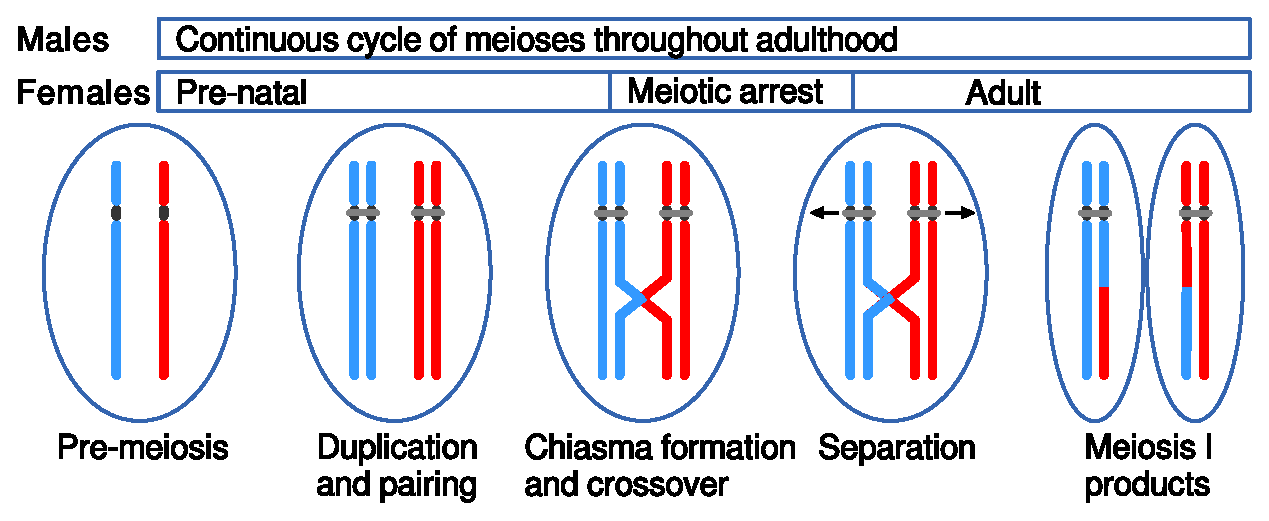
\includegraphics[width=\textwidth]{introduction/figs/meioticTiming}
    \end{center}
    \vspace{-10pt}
    \captionTitle{\textbf{Timing of meiosis I events in humans.}}{ 
        Males exhibit a continuous wave of meioses throughout adulthood.
        In females, meiosis begins before birth and enters an arrest period that can last decades before completion.
   \label{fig:introTiming}}
\end{figure}
\clearpage}


%%%%%%%%%%%%%%%%%%%%%%%%%%%%%%%%%%%%%%%%
%%%%%%%%%%%%%%%%%%%%%%%%%%%%%%%%%%%%%%%%
\section{Historical studies of meiotic recombination}
%%%%%%%%%%%%%%%%%%%%%%%%%%%%%%%%%%%%%%%%
%%%%%%%%%%%%%%%%%%%%%%%%%%%%%%%%%%%%%%%%

% Brief historical review of meiotic recombination, pre Human Genome Project.
Recombination can be observed in a number of ways, and its discovery came decades prior to the discovery of the structure of DNA.
Thomas Hunt Morgan first observed the separation of linked traits while studying Drosophila in 1911\cite{Morgan1911}, and proposed the theory of crossing over between chromosomes.
In addition he suggested that the recombination rate could increase with the distance between factors.
Morgan's student, Alfred Henry Sturtevant, quantified this change in rate over physical distance into ``map distance,'' using this concept to construct the first genetic map.
This map represented the order of, and crossover rates between genes on the X chromosome in Drosophila\cite{Sturtevant1913}.
In addition, Sturtevant observed that one crossover tended to inhibit the placement of a second nearby, an early description of interference.
A later study by Harriet Creighton and Barbara McClintock in corn (\textit{Zea mays}) in 1931 demonstrated that recombination between genes was tied to an exchange of chromosomal segments\cite{Creighton1931}.

Tracing the inheritance of markers from one generation to the next within a family pedigree provided the first genome-wide measurement of recombination across the human genome, prior to the completion of the Human Genome Project.
Early studies used restriction fragment length polymorphism (RFLP) probes to identify specific loci within the genome, and determine if they are linked.
An early study described the use of RFLPs to generate a linkage map of recombination in the human genome\cite{Botstein1980}.
Further linkage studies increased the marker density across the genome by using microsatellite, short tandem repeat polymorphisms (STRPs), and other approaches to capturing genetic variation\cite{Morton1991,Matise1994,Dib1996}.
The Marshfield map, generated in 1998 by \citet{Broman1998}, was an important step in characterizing recombination on a genome-wide basis.

With the completion of the Human Genome Project and the publication of the draft sequence of the human genome\cite{Venter2001,Lander2001}, human genetic variation has become increasingly well characterized.
As a consequence, a number of technologies have sprung up to make genome-wide ascertainment of variation a routine procedure.
Currently, microarray technology provides a well-balanced approach for determining genome-wide coverage of genetic variation.
These arrays target a pre-selected panel of hundreds of thousands to millions of single-nucleotide polymorphisms (SNPs) across every chromosome for a reasonable cost.

%%%%%%%%%%%%%%%%%%%%%%%%%%%%%%
\section{Methods for studying recombination}
%%%%%%%%%%%%%%%%%%%%%%%%%%%%%%

Genome-wide methods have the primary goal of creating a genetic map of the frequency of recombination as a function of physical distance across each chromosome.
Recombination is represented in units called Morgans, which quantify the amount of recombination between two physical locations, which are given in base pairs.
One Morgan corresponds to the physical distance between two markers so that an average of 1 crossover will occur between in any given meiosis.
Typically, the centiMorgan (cM) is the preferred unit of measurement, which is equivalent to 0.01 Morgans.
This data is used to generate genetic maps, which describe the relationship between genetic distance and physical distance on a chromosome.
In contrast to genome- or chromosome-wide methods, several other methods are limited in scope, and reveal information about specific loci.
With each method, the detection of recombination is made difficult by the fact that crossovers are rare -- only 20-60 are expected to occur in each meiosis.

% brief introduction to these before describing in detail in "description of approach"

\subsection{Pedigree analysis}

Tracking the transmission of alleles from one generation to the next within known pedigrees provided the first data on recombination in early linkage studies, and pedigree analyses are still widely in use today.
Regardless of the method used for obtaining markers, the principle of detecting recombination in a pedigree remains similar.
Crossovers can be identified by tracing the allele transmissions from parent to child.
Figure \ref{fig:introPedfig} provides a simple visual example, showing a family quartet.
The father in this pedigree has two informative SNPs producing haplotypes 1-1 and 0-0, while the mother is homozygous at both sites.
The male child has a 1-0 haplotype, and therefore must have inherited a recombinant haplotype from his mother.
We can identify here a crossover event and localize that event to an interval flanked by two informative genetic variants.
This region of uncertainty can vary in size and depends on the spacing and genotypes of polymorphic variants within the genome.
It is interesting to note that for a pedigree analysis, 
while whole-genome sequencing technology allows the discovery of a higher density of markers across the genome, its use is often not worth the higher cost.
A higher variant coverage will help to narrow the region of uncertainty surrounding a particular crossover, but it will most likely not assist in the detection of additional crossovers in a single meiosis.
Beyond this intuitive example, the problem of determining the parental phase of a recombinant chromosome has been addressed in a number of methods.
%
\afterpage{
\begin{figure}[p]
    \begin{center}
    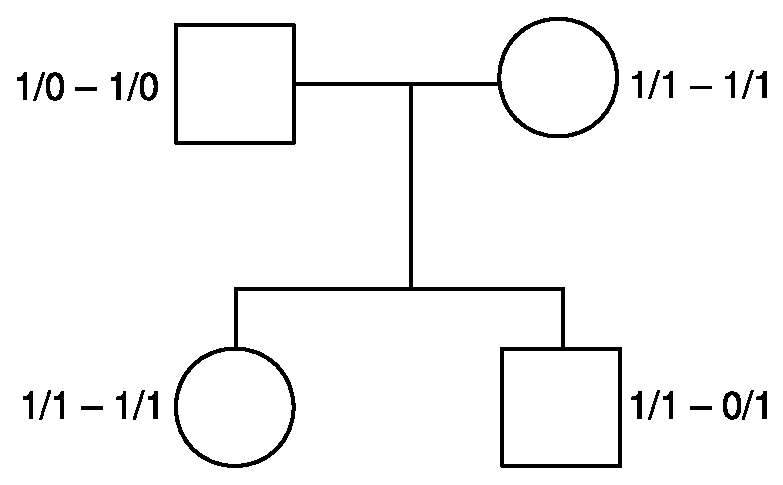
\includegraphics[width=0.75\textwidth]{introduction/figs/pedigree-genotype} \vspace{1cm} \\
    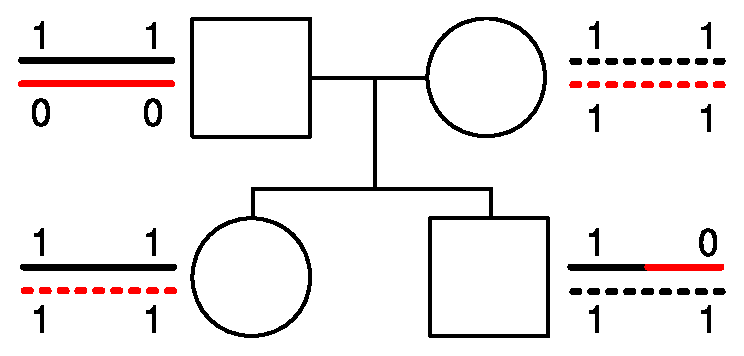
\includegraphics[width=0.8\textwidth]{introduction/figs/pedigree-haplotype}
\end{center}
    \vspace{-10pt}
    \captionTitle{\textbf{Allelic transmission in a family quartet.}}{ 
        The top panel outlines a simple pedigree in which only genotype information is known.
        The bottom panel shows a pedigree for which phase-known haplotype information is known.
        Here, all chromosomes (lines next to each individual) are transmitted in the absence of recombination except for in the male child.  Here there was a recombination event in the father to generate the recombinant chromosome (black/red)
   \label{fig:introPedfig}}
\end{figure}
\clearpage}


\subsection{Linkage disequilibrium approach}

Another powerful method uses population genetic data to study recombination.
These data can be gathered by genotyping samples from unrelated individuals on a microarray or by whole-genome sequencing.

The inference of recombination in such a dataset relies on the quantification of levels of linkage disequilibrium (LD) within the samples, a measurement of linkage between loci.
For example, when alleles at one locus are inherited completely independently of alleles at another locus they are considered to be in linkage equilibrium.
However, many alleles exhibit a non-random association, and individuals of the same species tend to share haplotype segments that reflect a shared evolutionary history.
When two alleles on an ancestral haplotype are inherited together they are considered linked, and are not independent of each other.
These alleles exhibit evidence of linkage disequilibrium, a deviation from the assumption of random assortment of alleles.

LD is measured in a pairwise fashion, considering allele frequencies at each pair of markers in the genome.
From measurements of LD within a number of unrelated samples, methods based on coalescent theory have been developed to estimate the recombination rate\cite{Auton2012}.
In software such as LDhat\cite{Mcvean2004,Auton2007,Auton2014}, the population-scale recombination rate, $\rho$, is estimated from the data, and the per-generation recombination rate can be calculated by the relationship
$\rho = 4 N_e r$
where $N_e$ represents the effective population size, and $r$ the per-generation recombination rate.
These methods are quite powerful and have produced high-quality estimates of recombination in humans\cite{hapmap2007}, however, they are subject to limitations.
First, this method requires the knowledge of the genealogical history of a sample, which is unknown, and thus relies on a simplifying approximation to the true genealogical structure.
Second, these maps by their nature generate sex-averaged data only, since recombination events that are inferred have occurred over the course of potentially thousands of generations.


\subsection{Molecular assays}

A number of molecular assays have been developed for studying recombination.
Most, however are limited to small regions of the genome, and are more effective in males.

\subsubsection{Sperm cell assays}

Sperm typing is one method of identifying both gene conversion and crossover events.
Sperm typing was first used in 1989 to study crossing over in humans\cite{Cui1989}, and uses
an allele-specific polymerase chain reaction (PCR) assay to identify recombination events at a given locus.
In this method, DNA is extracted from multiple haploid sperm cells from a single donor and subject to PCR.
A common reverse primer is used in conjunction with two different allele-specific forward primers, which correspond to a polymorphic site in the diploid genome, and are designed to produce different amplicon sizes depending on the matching nucleotide.
Analysis of the PCR products from many sperm cells can reveal the phase of the donor individual, and the recombinant status of each sperm cell.
% \cite{Jeffreys1998,Jeffreys2000,Jeffreys2004}. % first, second(TAP2), review

Sperm typing has been used to produce high-quality data from a number of loci throughout the genome.
One of the first major findings to come out of sperm typing was the characterization of recombination hotspots in the human major histocompatability complex (MHC), first within one gene, \textit{TAP2}\cite{Jeffreys2000}, then expanded to cover a wider 216 kb region of the MHC\cite{Jeffreys2001}.
All six hotspots found within the region of the MHC were found to be tightly correlated to regions in which LD broke down, providing molecular evidence that recombination hotpots have severe effects on LD patterns.


% Jeffreys2009: rise/fall
% Berg2010

Further work using whole genome, single-cell sequencing approaches has shed light on recombination on an individual basis for the first time.
A study by \citet{Lu2012} sequenced 99 sperm cells from an Asian male, providing valuable information on the level of variation across the entire genome of a single individual.
% Here,
In addition, a further study analyzed genome-wide recombination using more than 100 sperm cells\cite{Wang2012}.
These studies are promising, and when expanded to include measurements from multiple individuals, will provide much needed data on individual level variation in crossover, and potentially gene conversion as well.


\subsubsection{Single oocytes.}
Although much harder to study, recent studies have provided much needed insight into recombination in single oocytes through novel methods.
\citet{Hou2013} conducted an analysis in human oocytes, with the motivation to provide a potential new method for applying next generation sequencing methods to genetic screening with in vitro fertilization (IVF) techniques.
Here, the researchers extracted and fertilized a total of 70 oocytes from 8 Asian female donors, collecting the first and second polar bodies, as well as the male and female pronucleus from the fertilized egg.
This complete collection of data from female oogenesis and fertilization enabled complete haplotype phasing and crossover calls to be achieved.
Most intriguingly, this enabled the generation of personal genetic maps for each donor, allowing the researchers to address the question of how recombination varies on an individual basis.
This data allows the observation of all four members of the tetrad bundle, both sister chromatids and their homologues, something usually missed by inferential studies of recombination.


Using a similar approach, recovering genetic material from the first and second polar bodies and oocyte, \citet{Ottolini2015} were able to observe all four products of female recombination.
The researchers generated ``MeioMaps,'' providing valuable information on how meiosis proceeds on an individual level.



\subsubsection{Recombination initiation maps}
Additional methods have been developed to identify double strand breaks within a individual cells undergoing meiotic recombination.
\citet{Pratto2014} utilized chromatin immunoprecipitation coupled with sequencing to identify DSBs associated with the strand-exchange protein DMC1 to generate DSB maps in four unrelated human males.
This method identified the majority of DSBs within the meiotic cell, only a fraction of which would be resolved as crossovers that could be identified via genotyping methods.
The remainder would be repaired as non-crossover gene conversions.
The researchers found the DSBs cluster into hotspots, of which 51\% overlapped with the LD crossover hotspots\cite{hapmap2007}, and 80\% of DSB hotspots overlapped regions with elevated recombination rate.


% \section{Current ``gold standard'' maps (Hapmap2 LD map, deCODE pedigree map).}
\section{Genetic maps of recombination.}

\subsection{Marshfield map}
The Marshfield map, generated by \citet{Broman1998} in 1998, was the first genetic map of the human genome with a resolution high enough to make inferences on the recombination properties in humans, using $>$8,000 short tandem repeat polymorphsims (STRPs) in 188 meioses.
Here, estimates of the genome wide map lengths, inferences on individual variation, and sex differences in recombination were highlighted.
%% move to heterochiasmy?
The ratio of female to male autosomal map length was estimated at 1.56, indicating that the recombination rate in females is substantially higher than males.
This ratio has proved stable over a number of subsequent studies (summarized in Table \ref{tab:introHeterochiasmy}).
Analysis of this ratio as a function of chromosome position revealed that male recombination tends to be highest in the telomeres, while female recombination tends to be higher towards the centromeres.
This study provided valuable insight into broad-scale sex dimorphism in recombination, and raised questions as to the extent of fine-scale differences between males and females.

\subsection{deCODE maps}
Another major stride in pedigree-based genetic maps came from deCODE genetics, an Icelandic pharmaceutical company that used their database of genealogical and genetic data on many Icelandic families to infer recombination, producing several high quality studies.
The first was in 2002, in which 146 families, comprising 1,257 meioses, were genotyped using 5,136 microsatellite markers\cite{Kong2002}.
This data, in conjunction with the draft sequence of the human genome\cite{Venter2001,Lander2001} was used to improve the marker order and their placement within the reference sequence.
The genetic map generated from this study confirmed much found by \citet{Broman1998} in terms of sex dimorphism in recombination, and further characterized fine scale variation.
One particular finding was the discovery of recombination ``jungles,'' which are regions of high crossover rate that are clustered towards telomeres.
In addition, recombination rate was found to correlate with GC content, CpG motif occurrence, and tracts of poly(A)/poly(T), together explaining $\sim$37\% of variation.

In 2010, using genome wide SNP data, deCODE genetics published an updated sex-specific recombination map consisting of 15,257 meioses\cite{Kong2010}.
Instead of a typical pedigree-based recombination study, \citet{Kong2010} leveraged the high degree of relatedness within the Icelandic population to infer phase and parent-of-origin in 20,217 individuals typed on microarrays assaying $>$289,000 autosomal SNPs.
Here, phase was determined for parent-child pairs by taking into account haplotype blocks that are shared with other individuals within the population to determine the parent-of-origin for a particular block.
Crossovers were called when a segment of a child's haplotype was inferred to move between maternal and paternal origin.
This enables recombination be called in 15,257 parent-offspring pairs.
%%%
One effect of this parent-child phasing approach is that inference of recombination events near the telomeres was difficult, and \citet{Kong2010} omitted the most distal 5 Mb for each chromosome.
The omission of the telomeric regions, where male recombination is higher, contributed to the inflation of the female:male map length ratio, at 1.78 in this study.
The true value is more likely to be closer to the consensus ratio of around 1.6 (Table \ref{tab:introHeterochiasmy}).
Since its release in 2010 the deCODE genetic map has proven quite valuable as a high quality sex-specific map of recombination in the human genome.


\paragraph{Other pedigree studies.}
A study in 2008 performed a pedigree analysis of individuals from Hutterites, an isolated population of European descent that lives in the US\cite{Coop2008}.
This was the first study to use genome-wide high-density SNP arrays (in this case the Affymetrix GeneChip Mapping 500k array) to study recombination.
A total of 728 meioses were analyzed, yielding valuable data regarding the overlap of crossovers and hotspots on an individual basis.
Other pedigree studies include a map generated from 980 meioses using individuals of Korean and Mongolian descent\cite{Bleazard2013}.

\subsection{Linkage disequilibrium based maps}

LD has been used to great effect in the identification of recombination events, both in the human genome and in other species.
Perhaps the most high-quality LD map comes from data generated from the International Hapmap Project, Phase II\cite{hapmap2007}, which includes data from 270 individuals genotyped at over 3.1 million SNPs.
This map was generated using samples from both European (CEU) and African (YRI) origin, greatly improving the resolution over the Phase I map.
The resolution of this map refined the collection of hotspots first identified by \citet{Myers2005}, and expands this set to include 32,996 within the human genome.
This map remains in common use today, still providing the highest resolution of sex-averaged recombination rate across the human genome.
% ethnicity differences in these maps?


%%%%%%%%%%%%%%%%%%%%%%%%%%%%%%%%%%%%%%%%
%%%%%%%%%%%%%%%%%%%%%%%%%%%%%%%%%%%%%%%%
\section[Fine-scale recombination placement in the genome]{Fine-scale recombination placement in the genome: recombination hotspots}
%%%%%%%%%%%%%%%%%%%%%%%%%%%%%%%%%%%%%%%%
%%%%%%%%%%%%%%%%%%%%%%%%%%%%%%%%%%%%%%%%

\subsection{Initial discovery of recombination hotspots}

Sperm typing produced the first set of well-characterized hotspots in humans, initially focusing within the MHC\cite{Jeffreys2000,Jeffreys2001}.
Extensive analysis by sperm typing has indicated that hotspots can have recombination rates thousands of times that of the surrounding region and are generally just 1-2 kb in width\cite{Jeffreys2004a,Arnheim2003}.
The correlation of hotspot locations identified by sperm typing in this regions with the breakdown of LD measurements provided support for the use of LD methods to find hotspots of recombination genome-wide, without the expense and limitations of single-cell assays\cite{Jeffreys2001}.
Using LD methods\cite{Mcvean2004}, hotspots have been identified on genome-wide scales and in 2005 \citet{Myers2005} used LD methods to produce the first fine-scale recombination map of the human genome.
Using this map, hotspots were found to be a ubiquitous feature of the human genome, with over $\sim$25,000 hotspots identified, occurring roughly every 50 kb.
The subsequent HapMap LD map expanded the characterized set of hotspots to more than 30,000 throughout the human genome\cite{hapmap2007}.
These LD maps of recombination also estimated the proportion of recombination occurring within various fractions of the total genome sequence, finding that recombination was intensely concentrated, with 80\% of all recombination occupying less than 20\% of sequence.


\subsection{Discovery of PRDM9}

Since hotspots were first identified in large numbers, questions regarding the regulatory mechanism have persisted.
%the discovery that they were common and spread across the entire genome, 
\citet{Myers2005} found that DNA sequences within recombination hotspots were enriched for certain DNA repeat elements such as THE1A/B, as well as a short sequence motif (CCTCCCT) located at the centers of many hotspots.
A further family of motifs were identified via the use of the HapMap Phase 2 LD map\cite{hapmap2007}, encompassed by the degenerate 13 bp motif (CCNCCNTNNCCNC)\cite{Myers2008}, estimated to be involved in up to 40\% of all hotspots.
Hotspots were associated with increased GC content, GC increasing mutations, a likely result of the action of biased gene conversion\cite{Spencer2006}.


In 2010, a series of papers by three separate groups converged on the identification of PRDM9 from different approaches.
\citet{Myers2010} compared the sequence of the 13 bp motif against predicted binding of various zinc finger arrays in the genome, finding PRDM9 as a top candidate.
Using a mouse genetic approach, \citet{Baudat2010} focused on a locus previously determined to be involved in localization of crossover initiation\cite{Grey2009,Parvanov2009},
and narrowed this genomic interval to a region containing the \textit{Prdm9} gene.
A third study used linkage analysis in mice to narrow the region, again identifying PRDM9 as the likely candidate protein\cite{Parvanov2010}.

PRDM9 was originally identified in mice, where is was called \textit{Meisetz}, and was shown to be active only in early meiotic prophase\cite{Hayashi2005}.
PRDM9 (PR domain containing 9) has multiple domains.
It contains a KRAB (Kruppel-associated box) domain, that is potentially involved in protein-protein interactions, a PR/SET domain that serves a methyltransferase function, responsible for the trimethylation of lysine 4 on histone 3 (H3K4)\cite{Hayashi2005}.
PRDM9 also contains a high polymorphic C2H2 zinc finger array, responsible for binding to specific DNA sequences\cite{Hayashi2005}. 

\subsection{PRDM9 alleles}

The PRDM9 zinc finger array has tremendous variability and there are a number of alleles present, not just in humans but also chimpanzees and other primates\cite{Schwartz2014}.
In humans, the major alleles A and B, are both present in a high percentage of European individuals, and differ by only a single amino acid change, while the I allele encodes a longer zinc finger array\cite{Baudat2010}.
The A and B alleles are predicted to recognize the degenerate 13-mer motif, but the I allele is not\cite{Baudat2010}.
This effect is seen at the DSB-level as well, with PRDM9 A and B variants contributing to generate similar DSB hotspots\cite{Pratto2014}.

Furthermore the PRDM9 allele status of an individual has a strong effect on the hotspot overlap.
In the Hutterite study, A/A individuals have significantly different overlap compared to A/I, and A/B, with the A/I heterozygous having lower hotspot usage overall\cite{Baudat2010}.

Sperm typing in men of African ancestry revealed that PRDM9 variants similar to the ``C'' allele (termed C-type), were more common in this population.
Furthermore, these C-type alleles specified different hotspots with a motif different from those seen Europeans\cite{Berg2011}. 
These ``African-enhanced hotspots'' all contained a common motif, CCNCNNTNNNCNTNNC, but were associated with the PRDM9 C-type alleles.

A study using recombination initiation maps of recombination to locate DSBs found that PRDM9 alleles affected DSB locations, which represent a set of both crossovers and gene conversion\cite{Pratto2014}.
The DSB locations were largely tied to the specific PRDM9 allele for each particular individual.
PRDM9$_\text{A}$ and PRDM$_\text{B}$ alleles appear to specify similar DSB hotspots, while PRDM9$_\text{C}$ has a separate specificity.
PRDM9 heterozygosity was also found to influence hotspot strength.


%%%%%%%%%%%%%%%%%%%%%%%%%%%%%%%%%%%%%%%%
%%%%%%%%%%%%%%%%%%%%%%%%%%%%%%%%%%%%%%%% move from other species to here
% PRDM9 is a rapidly evolving gene and is under high selective pressure across a wide variety of species\cite{Oliver2009,Ponting2011}.


%%%%%%%%%%%%%%%%%%%%%%%%%%%%%%%%%%%%%%%%
%%%%%%%%%%%%%%%%%%%%%%%%%%%%%%%%%%%%%%%%
%\section{Determinants of broad-scale localization of recombination in the genome.}
%%%%%%%%%%%%%%%%%%%%%%%%%%%%%%%%%%%%%%%%
%%%%%%%%%%%%%%%%%%%%%%%%%%%%%%%%%%%%%%%%
%%%%%%%%%%%%%%%%%%%%%%%%%%%%%%
%%%%%%%%%%%%%%%%%%%%%%%%%%%%%%
\section{Sexual dimorphism in recombination}
%%%%%%%%%%%%%%%%%%%%%%%%%%%%%%
%%%%%%%%%%%%%%%%%%%%%%%%%%%%%%
% Differences in populations (Berg2010,Berg2011,Hinch2011)

\subsection{Broad scale distribution within the genome differs between the sexes}

The distribution of recombination within the genome varies considerably between individuals, sexes, and populations.
At the broad scale, crossovers are not distributed equally across the genome.
The recombination rate is higher towards the telomeres\cite{Broman1998,Mcvean2004,hapmap2007}.
This effect seems to be primarily driven by sex.
Crossing over in males occurs more frequently in telomeric regions, while females have higher recombination rates closer to the centromeres\cite{Kong2002,Coop2008,Kong2010}.

Numerous studies in humans have found that recombination tends to be depressed within gene regions overall, with high recombination just upstream and downstream of gene regions\cite{Mcvean2004,Myers2005,hapmap2007,Spencer2006,Kong2010}.
When looking further away from gene regions, recombination appears to be elevated up to around around 500 kb away, then falls off after a few hundred kb more.
Evidence for sex differences in recombination has also been suggested to occur around gene regions.
\citet{Kong2010} found that recombination was lower within genes overall, and that
female recombination was lower within genes, but higher in the surrounding regions.
Additionally, while females have a lower rates within genic regions, males have higher rate within exonic regions\cite{Kong2010}.

In addition, results from LD maps in humans have examined the proportion of recombination occupying various proportions of sequence.
From these analyses, it is estimated that the majority of recombination, 80\%, occurs in approximately 20\% of the sequence\cite{Mcvean2004,Myers2005,hapmap2007}
This concentration of recombination could be due to clustering within hotspots.
A majority of crossovers in each meiosis were found to cluster into recombination hotspots, driving recombination into limited region of the genome\cite{Coop2008}, although this overlap varies widely between individuals.


\subsection{Recombination under genetic control}
% Genes involved in recombination (RFN212, etc)}

A number of genetic factors have been identified that alter properties of recombination, a summary of which can be found in Table \ref{tab:introGenes}.
In a sperm typing analysis, \citet{Jeffreys2005} found a SNP whose minor allele suppressed the ratio of crossover to gene conversion near a particular hotspot.
Additionally, this variant was found to be overtransmitted in the offspring.
This is an example of meiotic drive, in which forces acting during meiosis alter the expected transmission ratios for a particular locus, causing over- or under-transmission.
Another study in the Icelandic population found an association with an inversion at 17q21.31 on recombination rate\cite{Stefansson2005}.
The presence of this inversion is associated with an increase in crossover rate in females, but not males.

% RNF212: indentified in Saccharomyces cerevisiae and Caenorhabditis elegans
In addition, RNF212 has been associated with recombination rate in an Icelandic population\cite{Kong2008}, and this has been replicated in a number of follow-up studies\cite{Chowdhury2009,Fledel-Alon2011,Reynolds2013,Kong2014}.
Interestingly, the linkage of two particular SNPs near this gene is associated with an increased recombination rate in males, and a corresponding decreased rate in females.
RNF212 is a homologue of ZHP-3, a \textit{C.\ elegans} gene involved in crossing over and disjunction, localizing to sites of crossover, and aids in the change in chromatin structure that occurs with the disassembly of the synaptonemal complex\cite{Bhalla2008}.
Mouse RNF212 was found to have similar function, facilitating synapsis, and forming crossover-stabilizing structures\cite{Reynolds2013}.
%Rnf212 KO mice are sterile but achieve complete synapsis.
In addition RNF212 possibly influences the decision to repair a DSB as a crossover rather than a gene conversion\cite{Reynolds2013}.

A study by \citet{Chowdhury2009} using 2,310 meioses found significant associations with variants associated with four gene regions.
Two were associated with female recombination rate (KIAA1462, PDZK1), and the other two with male rate (UGCG, NUB1).
These genes are poorly characterized and their function, beyond potential meiotic roles, remains unknown.
However, this study reinforces the suggestion that male and female recombination rate are controlled via differing genetic factors.

Another study, again in the Icelandic population with an expanded number of meioses, identified a further 8 genomic regions that have separate associations with male and female recombination rates\cite{Kong2014}.
In the telomeric region of chromosome 4, near RNF212, one variant was found that was estimated to increase the map length by 386 cM in females, and 124 cM in males.
Novel variants were found in an additional six genes (Table \ref{tab:introGenes}).

The strongest association thus far has been with the PRDM9 protein, which was first associated with hotspot usage and variation in alleles encoding the zinc finger array\cite{Baudat2010,Berg2010}.
\citet{Berg2011} found that DNA sequence variation in \textit{PRDM9} alleles greatly influences hotspot usage in African populations, who appear to have a distinct subset of hotspots\cite{Hinch2011}.
Genome-wide associations with hotspot usage were replicated in the Icelandic population with strong effects\cite{Kong2010}.

In non-human studies, both RNF212, and REC8, a SC-associated protein, have also been shown to associate with recombination rate in cattle\cite{Sandor2012}.
%
\afterpage{
\begin{table}[p] \centering
    \small
    \begin{tabular}{|l|c|c|p{1.3cm}|p{1.3cm}|c|c|} 
\hline Gene / region & Chr. & Association & Female rate & Male rate & Study & Replication \\ \hline
\rule{0pt}{2ex}   RNF212 & 4 & rate & + & - & \citet{Kong2008} & \cite{Chowdhury2009,Fledel-Alon2011,Reynolds2013,Kong2014,Campbell2015} \\
        17q21.31 inversion & 17 & rate & + & none & \citet{Stefansson2005} & \cite{Fledel-Alon2011,Chowdhury2009,Kong2014} \\
        KIAA1462 & 10 & rate & + & none & \citet{Chowdhury2009} &  \\
        PDZK1 & 1 & rate & + & none & \citet{Chowdhury2009} &  \\
        UGCG & 9 & rate & none & + & \citet{Chowdhury2009} &  \\
        NUB1 & 7 & rate & none & + & \citet{Chowdhury2009} &  \\
        CCNB1IP1 & 14 & rate & + & weakly + & \citet{Kong2014} & \cite{Campbell2015} \\
        C14orf39 & 14 & rate & + & none & \citet{Kong2014} &  \\
        SMEK1 & 14 & rate & + & none & \citet{Kong2014} & \cite{Campbell2015} \\
        RAD21L & 20 & rate & weakly + & + & \citet{Kong2014} &  \\
        MSH4 & 1 & rate & + & none & \citet{Kong2014} &  \\
        CCDC43 & 17 & rate & + & none & \citet{Kong2014} &  \\
        PRDM9 & 5 & hotspot usage & NA & NA & \citet{Baudat2010} & \cite{Fledel-Alon2011,Campbell2015,Kong2014} \\
    \hline \end{tabular}
    \captionTitle{\textbf{Genomic regions associated with recombination in humans.}}{
    \label{tab:introGenes}}
\end{table}
\clearpage}

\paragraph{Heritability of recombination modifiers.}
Several lines of evidence indicates that modifiers of recombination are heritable.
In the 2004 deCODE study, siblings in large families, were analyzed and data suggested that recombination rates are broadly heritable\cite{Kong2004}.
The pedigree analysis of the Hutterites population by \citet{Coop2008} was the first to find extensive DNA sequence variation among individuals in terms of their hotspot overlap (the proportion of an individual's crossover that overlap with known hotspots).
Furthermore, it was found that the extent that hotspots overlap is also heritable.
Further work reinforced the heritability of hotspot usage as a phenotype, and supported the finding that both male and female recombination rates are heritable\cite{Fledel-Alon2011}.
In addition, selection has been shown to act to retain eggs with higher recombination rates\cite{Ottolini2015}, a phenomenon previously suggested to explain the apparent increase in recombination rate in older mothers\cite{Kong2004}.
This raises the possibility that other aspects of the recombination process may also be heritable, but further work in larger cohorts is will necessary to determine the full extent of these modifiers.


%%%%%%%%%%%%%%%%%%%%%%%%%%%%%%
%%%%%%%%%%%%%%%%%%%%%%%%%%%%%%
%\section{Sexual dimorphism in recombination.}
%%%%%%%%%%%%%%%%%%%%%%%%%%%%%%
%%%%%%%%%%%%%%%%%%%%%%%%%%%%%%
\subsection{Heterochiasmy}

\afterpage{
\begin{table}[p] \footnotesize
    %\begin{tabular}{|P{3.2cm}|c|c|p{1.6cm}|p{1.3cm}|c|p{1.7cm}|} 
    \begin{tabular}{|P{3.2cm}|c|c|c|c|c|c|} 
        \hline Common name (species) & Year & Study & Female (cM) & Male (cM) & Ratio & Sex avg (cM) \\ \hline
\rule{0pt}{2ex} Human (\textit{Homo sapiens}) & 1991  & \citet{Morton1991} & 4782 & 2809 & 1.70 & 3795.50 \\
       & 1994  & \citet{Matise1994} & 4790 & 2625 & 1.82 & 3707.50 \\
       & 1996  & \citet{Dib1996} & 4198.8 & 2729.7 & 1.54 & 3464.25 \\
       & 1998  & \citet{Broman1998} & 4251 & 2730 & 1.56 & 3490.50 \\
       & 2000  & \citet{Broman2000} & 4435 & 2730 & 1.62 & 3582.50 \\
       & 2002  & \citet{Kong2002} & 4280.9 & 2590.5 & 1.65 & 3435.70 \\
       & 2008  & \citet{Coop2008} & 4133 & 2699 & 1.53 & 3416.00 \\
       & 2010  & \citet{Kong2010} & 4070.8 & 2286.6 & 1.78 & 3178.70 \\
       & 2013  & \citet{Bleazard2013} & 3933.5 & 2502.9 & 1.57 & 3218.20 \\
       & 2014  & \citet{Kong2014} & 3868 & 1925 & 2.01 & 2896.50 \\
       & 2015  & \citet{Campbell2015} & 4354.91 & 2707.66 & 1.61 & 3531.29 \\
       & 2016  & \citet{Bherer2016} & 4122.8 & 2635.2 & 1.56 & 3379.00 \\ \hline
\rule{0pt}{2ex} Mouse (\textit{Mus musculus}) & 2009  & \citet{Cox2009} & 1495.3 & 1375.3 & 1.09 & 1435.30 \\ \hline
\rule{0pt}{2ex} Dog (\textit{Canis lupus familiaris})* & 1997 & \citet{Mellersh1997} & 1039 & 766 & 1.36 & 902.50 \\
     & 1999 & \citet{Neff1999} & 1820 & 1290 & 1.41 & 1555.00 \\
     & 2010 & \citet{Wong2010} & 2276 & 1909 & 1.19 & 2092.50 \\
     & 2016 & Chapter \ref{ch:dogPed} & 2162 & 1816 & 1.19 & 1989.00 \\ \hline
\rule{0pt}{2ex} Sheep (\textit{Ovis aries}) & 1995 & \citet{Crawford1995} & 1907 & 2143 & 0.89 & 2025.00 \\ \hline
\rule{0pt}{2ex} Cattle (\textit{Bos taurus}) & 1997 & \citet{Kappes1997} & 2879 & 2808 & 1.03 & 2843.50 \\
        & 2015 & \citet{Ma2015} & 2320 & 2550 & 0.91 &  \\ \hline
\rule{0pt}{2ex} Pig (\textit{Sus scrofa}) & 1995 & \citet{Archibald1995} & 2150 & 1650 & 1.30 & 1900.00 \\
     & 1996 & \citet{Marklund1996} & 2565 & 1830 & 1.40 & 2197.50 \\ \hline
\rule{0pt}{2ex} Short-tailed opossum (\textit{Monodelphis domestica})* & 2004 & \citet{Samollow2004} & 443.1 & 884.6 & 0.50 & 663.85 \\ \hline
\rule{0pt}{2ex} European tree frogs (\textit{Hyla arborea})* & 2008 & \citet{Berset-Brandli2008} & 296.6 & 20.7 & 14.33 & 158.65 \\ \hline
\rule{0pt}{2ex} Zebrafish (\textit{Danio rerio})* & 2002 & \citet{Singer2002} & 2582.7 & 942.5 & 2.74 & 1762.60 \\ \hline
\rule{0pt}{2ex} Rainbow trout  & 2000 & \citet{Sakamoto2000} &  &  & 3.25 &  \\
(\textit{Oncorhynchus mykiss})* & 2005 & \citet{Danzmann2005} &  &  & 4.31 &  \\ \hline
\rule{0pt}{2ex} Arctic charr (\textit{Salvelinus alpinus})* & 2005 & \citet{Danzmann2005} &  &  & 1.69 &  \\ \hline
\rule{0pt}{2ex} Atlantic salmon (\textit{Salmo salar})* & 2005 & \citet{Danzmann2005} &  &  & 16.81 &  \\ \hline
\rule{0pt}{2ex} Pigeon (\textit{Columba livia})* & 1999 & \citet{Pigozzi1999} &  &  & $\sim$equal &  \\ \hline
\rule{0pt}{2ex} Chicken (\textit{Gallus gallus domesticus})* & 2009 & \citet{Groenen2009} & 3097.7 & 2913.7 & 1.06 & 3005.70 \\ \hline
\rule{0pt}{2ex} Great reed warbler (\textit{Acrocephalus arundinaceus})* & 2005 & \citet{Hansson2005} & 237.2 & 110.2 & 2.15 & 173.70 \\ \hline
\rule{0pt}{2ex} Fruit fly (\textit{Drosophila melanogaster})* & 1914 & \citet{Morgan1914} &  & no rec. & NA &  \\ \hline
\rule{0pt}{2ex} Arabadopsis (\textit{Arabidopsis thaliana}) & 2013 & \citet{Basu-Roy2013} & 332 & 575 & 0.58 & 453.50 \\
    \hline \end{tabular}
    \captionTitle{\textbf{Autosomal map length estimates in various species.}}{
        Total map lengths are given in centimorgans, while the ratio represents the female to male map lengths. Some studies do not provide map lengths but ratios are reported here as they are found in the text. PRDM9-absent species are marked with an asterisk (*).
\label{tab:introHeterochiasmy}}
\end{table}
\clearpage}

The Marshfield map\cite{Broman1998}, provided some of the first genome wide evidence of recombination rate variation across the human genome, and between males and females.
Particularly interesting was the finding that recombination rates are higher in the telomeres, especially in males, and that females have a 1.56-fold higher rate of recombination in the autosomes.
The estimation of this ratio proved to be accurate, despite the low marker coverage and few meioses used, and has been reinforced through numerous follow-up studies\cite{Broman2000,Kong2002,Coop2008,Kong2010,Bleazard2013,Campbell2015,Bherer2016}. % (Table \ref{tab:introHeterochiasmy}).

This example in humans provides an illustration of heterochiasmy, the unequal distribution of recombination rates between the sexes of a species.
Humans are among a large majority of species with data currently available in which the female recombination rate is higher than that of the male (Table \ref{tab:introHeterochiasmy}).

Related to heterochiasmy is the Haldane-Huxley rule\cite{Haldane1922,Huxley1928}, which states that in organisms in which one sex has an absence of recombination (achiasmate) it is the heterogametic sex (the sex with differing sex chromosomes, e.g.\ XY males).
Because recombination is suppressed between the sex chromosomes in the heterogametic sex, \citet{Haldane1922} hypothesized that this suppression carried over to the autosomes as well.
But the Haldane-Huxley rule does not apply to species in which neither sex is achiasmate.
There are a number of known species in which the heterogametic sex has an equal or higher recombination rate than the homogametic sex (e.g.\ XX females), and several other possibilities have been proposed.

One interesting explanation is that recombination is lower in the sex that undergoes stronger selection.
% recombination is suppressed in males because there is less selective pressure to do so\cite{Trivers1988}.
\citet{Trivers1988} suggested that males in general are subject to stronger selective forces than females, who often have more choice in their selection of a mate.
Because males with very fit phenotypes reproduce more often that unfit males, these males will tend to keep their high-fitness gene combinations because disrupting these favorable haplotypes will be selected against.
%there is less selective force to recombine.
In contrast, females do not have as much variability in their ability to reproduce and selective pressure is lower.
% (recombination disrupts favorable haplotypes in the most fit individuals, therefore is selected against).

This idea has been criticized however, especially because selection in an adult, diploid organism is unlikely to affect recombination rate at the haploid stage\cite{Lenormand2003}.
\citet{Lenormand2005} suggested that haploid selection may act differently in males and females and that this, and not heteromorphic sex chromosomes, could account for the heterochiasmy observed in plants.
A more recent study\cite{Otto2015} supports this idea, suggesting an additional level of parental control over the level of selection experienced by a given gamete.

In mammals, the idea of haploid selection to effect dimorphism is an attractive one to explain heterochiasmy, although the strength of selection is markedly lower.
Since oogenesis is arrested at dictyotene and does not complete until fertilization, the haploid stage is essentially absent in females.
Therefore, there is a higher potential for selection in male haploids, even if only a handful of genes are actually expressed\cite{Dadoune2004}.
In addition, there is evidence for elevated female recombination rates in imprinted regions\cite{Lercher2003}, which further confounds this issue of male or female control over haploid selection.

In most studied species, including humans, females have a higher rate and a longer map length than males, with a ratio ranging from just above 1, to 14 in the European tree frog\cite{Berset-Brandli2008}, and nearly 17 in Atlantic salmon\cite{Danzmann2005}.
Estimates in humans, perhaps the most well studied organism, have demonstrated little variation since the earliest linkage studies, with a ratio of 1.6.

However, the heterogametic sex does not always have a lower recombination rate.
A number of species have roughly equivalent rates of recombination between the sexes, including pigeons\cite{Pigozzi1999} and possibly cattle\cite{Kappes1997}. %, although a more recent study suggested that male cattle may actually have a higher rate than females\cite{Ma2015}.  
Indeed, many species have higher recombination rates in males.
Sheep\cite{Crawford1995} (0.89), and a more recent study in cattle\cite{Ma2015} (0.91), demonstrate only slightly higher rates in males.
However, marsupials provide the most extreme example. 
In the short-tailed opossum\cite{Samollow2004},  males have twice the amount of recombination as females (a ratio of 0.5).

%%%%%%%%%%%%%%%%%%%%


Cytological studies of meiotic cells have provided convincing evidence that the sex differences in crossover count are driven by, or parallel differing chromatin configurations across meiotic prophase.
Using molecular cytological studies, the entirely of the SC can be visualized and measured with markers to SYCP3, which is a transverse element protein.
The SC is substantially longer in females than males, translating to a correspondingly larger DNA loop size\cite{Tease2004,Gruhn2013}.
This relationship has been proposed to account for the differences in crossovers observed between males and females.
Males and females have chromosomes of identical size (among the autosomes), so packaging the same amount of DNA into a smaller total SC length would naturally mean a larger loop size.
In addition males have fewer DSBs overall, when examining markers for RAD51, which associate with DSBs, indicating that these differences occur prior to or at the onset of DSB formation\cite{Gruhn2013}.
There is also evidence for variation in the SC length for chromosome arms, suggesting that SC length depends on the chromatin configuration for each chromosome arm and not the physical length\cite{Codina-Pascual2006a}.

%%%%%%%%%%%%%%%%%%%%%%%%%%%%%%
\subsection{Conflicting evidence for a maternal age effect on recombination rate.}
%%%%%%%%%%%%%%%%%%%%%%%%%%%%%%

Age effects on reproduction have been tied with an increased incidence of aneuploidy in humans\cite{Hassold2001,Hassold2007}.
Over the past decade, several studies have provided conflicting reports on an association of recombination rate and maternal age.
Those that have demonstrated an increase in the number of crossovers with maternal age suggest that this increase could be a protective mechanism against aneuploidy.

%%%
With the aim of investigating age effects in recombination, a study in 2004 used the deCODE genetics dataset with 23,066 meioses, with a reduced set of 1000 microsatellite markers\cite{Kong2004}.
Genotyping was not done for every individual, with some families having only one parent genotyped, and recombination events were therefore imputed.
The main finding from this study is that the number of crossovers observed in females appears to increase with age, with an additional 0.082 events per year ($\pm$0.012), corresponding to a 4\% increase over 25 years.
This effect was seen to increase within families, such that a child born later in the mother's life has a higher number of maternal crossover than their siblings born earlier.
\citet{Coop2008} analyzed recombination in 728 meioses from Hutterites, and found that mothers 35 year or older have an extra 3.1 crossover events compared to mothers under 25 years old.
This effect corresponds with an extra 0.19 events per year ($\pm$0.092).
No such effect was found in males in either study.
%%%

A study by \citet{Hussin2011} examined in recombination in 195 maternal meioses from French-Canadian pedigrees.
Here, the opposite effect was seen, with recombination rate found to decrease with maternal age, with a larger effect size.
The crossover count was estimated to decrease by $-$0.49 to $-$0.42 events each year.
Differences in the direction of the effect here may be due to real differences between populations, when considering the French-Canadian population as a genetic isolate, or simply due to a lack of power with only 195 meioses.
%%%
Another study reported a slight decrease in crossover count with maternal age in 338 meioses, finding a decrease of $-$0.29 events per year\cite{Bleazard2013}.

% In a direct test of the production line hypothesis, \citet{Rowsey2014} examine more than 8,000 oocytes, finding no significant change in crossover count among oocytes.
% Thus, it appears that the number of crossovers in a given oocyte is not controlled as a function of order of meiotic entry, and there is a lack of evidence for any effects of the production line hypothesis on crossover count.

While evidence for an age effect on crossover count in females is conflicting, these studies all agree that there is no age effect present in males.
A recent multi-cohort analysis by \citet{Martin2015} provided much need insight into the age effect issue.
Using a combination of nine cohorts comprising $>$6,000 meioses, the authors report a modest but significant increase in the crossover count with age.
The authors used a comprehensive and systematic approach that avoids the methodological differences between previous studies.
%%%
An interesting suggestion from this study was that of possible confounding factors upon the maternal age effect.
First, that assisted reproductive technologies, including IVF, may provide an artificial selection for oocytes with a greater number of crossovers.
Second was the possibility that oral contraception, which suppresses ovulation, could somehow alter the age-count association. %, especially if the production-line hypothesis holds true for humans.
However, neither of these possibilities could be controlled for with the power of this study and remain undetermined.

Several other studies approach this question from another direction.
Evidence in mice point to sex differences in cell cycle checkpoints that control for, and terminate cells with excessive DNA damage, or without chiasmata\cite{Cohen2006}.
The first of at least two checkpoints in prophase I is triggered by lack of synapsis, or breaks in the DNA that have been missed by repair machinery.
A second checkpoint, in late pachytene, senses chromosomes without chiasma, and female mice appear to frequently bypass this checkpoint, while male mice do not.
Thus is appears that female mice may have a less stringent set of checkpoints, and that this may account for the increased incidence of meiotic abnormalities\cite{Cohen2006}.

An analysis of single oocytes provides evidence that maternal recombination rate is highly variable within a single individual, with 41.6 $\pm$ 11.3 crossover per oocyte\cite{Ottolini2015}.
This study revealed a selection against transmission of non-recombinant oocytes at meiosis II.
These achiasmate products were more likely to be found in the second polar body instead of the transmitted oocyte.
This evidence outlines a potential mechanism by which non-recombinant, potentially aneuploid oocytes could be eliminated from the germ line.
Furthermore, recombination, thought to be limited to prophase I, was shown to influence events in meiosis II, much later than previously thought.

\subsection{Open questions in sexual dimorphism in recombination}
Taken together, this evidence reflects a tremendous variation in levels of sexual dimorphism and heterochiasmy, both across and within species, as well as on an individual basis.
From recombination surveys of various species, it is clear that heterochiasmy manifests itself in a number of different ways.
Cytological evidence shows that differences in recombination rate are related to changes at the molecular level, a result of the differing mechanisms for completing meiosis between males and females.
In addition, aging effects on the recombination process point to a carefully regulated process that has potential to degrade with time.
One possibility is that biological differences in the meiotic process could drive the differences in recombination outcomes.
Alternatively these differences could arise as a product of the differing requirements imposed upon recombination between the sexes by external forces such as natural selection.
Though much work has been done, both theoretical and experimental, no clear explanations have emerged, and the question of the cause of heterochiasmy and differences between the sexes in the recombination process remain unanswered.
These questions will be addressed within this thesis, for humans in Chapters \ref{ch:cointEsc} and \ref{ch:cointExtras}, and for dogs in Chapter \ref{ch:dogPed}.




%%%%%%%%%%%%%%%%%%%%%%%%%%%%%%%%%%%%%%%%
%%%%%%%%%%%%%%%%%%%%%%%%%%%%%%%%%%%%%%%%
\section{Recombination and disease}
%%%%%%%%%%%%%%%%%%%%%%%%%%%%%%%%%%%%%%%%
%%%%%%%%%%%%%%%%%%%%%%%%%%%%%%%%%%%%%%%%

\subsection{Non-disjunction and the role of recombination.}

In humans, aneuploidy is a major cause of pregnancy loss and disease.
An estimated 30\% of fertilized eggs have aneuploid chromosomes\cite{Hassold2001}.
The incidence of aneuploidy remains at a low baseline level in individuals in their twenties, with males having 1-4\% and females 2-3\% of their sperm or eggs with aneuploidy\cite{Hassold2009,Nagaoka2012}.
This number rises steeply with age in females, up to 35\% or more\cite{Nagaoka2012}.
%Males in their twenties have a baseline level of aneuploid sperm of 1-4\%, while females have 2-3\%, a number that rises sharply with maternal age\cite{Hassold2009,Nagaoka2012}.
Aneuploidy in newborns (0.3\%) and stillbirths (4\%) is relatively rare compared to the rate of aneuploidy in spontaneous abortions, which can be more than 35\%\cite{Nagaoka2012}.

Multiple lines of evidence have suggested that meiotic errors are responsible in many cases.
Non-disjunction, the abnormal segregation of chromosomes, can occur at either of the two cell divisions in meiosis.
Meiosis errors can occur in both males and females, but errors are much more frequent in females\cite{Hassold2001,Nagaoka2012}.
Meiosis I non-disjunction is thought to involve recombination, either in a failure to resolve chiasmata, or a lack of chiasmata entirely.
Several genomic disorders have been linked to meiosis I errors, which are a common cause of trisomies of chromosomes 15, 16, 21, and 22 in females\cite{Nagaoka2012,Hassold2001}.
Meiosis II non-disjunction typically results from a failure of the sister chromatids to separate, which is frequently caused by achiasmate chromosomes.
This complete lack of crossover is a frequent cause of female trisomy 18\cite{Nagaoka2012}.
In males, meiosis I errors are frequent in trisomy 2, and in Klinefelter syndrome (47,XXY), while meiosis II errors contribute to trisomies of chromosomes 14 and 15\cite{Hassold2007}.


A reduced recombination rate has been observed in human genetic maps generated from viable meiosis I aneuploidies (15, 16, 18, 21, XXX, XXY)\cite{Hassold2001,Lynn2004}.
This indicates that recombination rate must remain above a certain level to prevent non-disjunction.
This is supported by the finding that many trisomies involve achiasmate chromosomes, in which recombination is absent in that chromosome\cite{Nagaoka2012}.

This supports the idea that chiasmata, which serve to tether homolgous chromosomes together after the dissolution of the SC, and through the end of anaphase I, provide a crucial tension that serves to inhibit non-disjunction.
Research suggests that there is a requirement of one chiasma per chromosome to prevent non-disjunction, but that there may be a backup mechanism to enable chromosomes to properly segregate even without any chiamata\cite{Fledel-Alon2009}.

Meiotic arrest of oocytes in mammals has been the subject of much discussion because it may be associated with increased aneuploidy in humans, in particularly in older mothers.  
Several biological possibilities have been proposed to explain what happens to oocytes during meiotic arrest.
One is the production line hypothesis, first proposed in 1968\cite{Henderson1968}, which proposes that oocytes exit meiosis and are ovulated in the order in which they enter.
An implication of this is that an oocyte produced early in the fetal stage, which will thus exit early, must have more robust crossover connections and are less prone to aneuploidy when compared to later oocytes.
This may explain why aneuploidy occurs more frequently in older mothers.
Furthermore, the production line hypothesis suggests that chiasmata frequency would decrease with age in females, as the rate of aneuploidy increases.
Several tests of the production line hypothesis have been done in mammals.
There is evidence to support the existence of a production line in mice\cite{Polani1991}, suggesting that oocytes exit meiosis in the order in which they enter.
However several studies in humans contradict the assumption of a decrease in crossover count in older mothers\cite{Kong2004,Martin2015}.
In a direct test of the production line hypothesis in humans, \citet{Rowsey2014} examine more than 8,000 fetal oocytes, finding no significant change in crossover count.
Thus, it appears that the number of crossovers in a given oocyte is not controlled as a function of order of meiotic entry, and there is a lack of evidence for any effects of the production line hypothesis on crossover count.

Another possibility, suggested by a study in the Icelandic population\cite{Kong2004}, is oocytes that have higher recombination rates are more likely to survive to become successful embryos.
Since a higher rate of recombination is linked to a lower incidence of aneuploidy, it is possible that oocytes with lower crossover counts were more likely to be aneuploid.
These aneuploid oocytes would therefore be discarded somehow, by a cell cycle checkpoint mechanism for example.
These could not be observed in a study looking at presumably healthy, or at least viable, offspring and would giving the impression of a recombination rate increase.

%%% other possibilities? rec events during arrest period.

\subsection{Genomic instability}
The most direct association of recombination with disease is with aneuploidy due to meiosis I errors\cite{Hassold2001,Hassold2007}.
Otherwise, since recombination has such a high impact on the structure of the genome, it also has the possibility to cause genomic instability if errors occur during the break and repair of DNA.
Defects in recombination have been associated with a number of disorders caused by genomic instability.
Errors in the repair of breaks initiated during recombination are a major cause of structural variants, leading to disease\cite{Carvalho2016}.
Nonallelic homologous recombination (NAHR), also known as ectopic exchange results in structural genomic rearrangements and is a major cause of recombination-associated copy number alteration.
This occurs in locations in the genome containing segmental duplications, also referred to as low copy repeats (LCRs).  
These blocks of sequence evolved recently in primate evolution and are highly homologous.
Unequal exchanges can be caused due to non-allelic recombination between different, paralogous LCRs.  
For example, 22q11.2 deletion syndrome is believed to be caused by improper pairing and crossing over between LCR22s that flank the region, causing it to be deleted in the recombinant chromosome\cite{Emanuel2008}.

Ectopic exchange contributes to a number of other similar types of genomic diseases associated with LCR-mediated rearrangements\cite{Stankiewicz2002,Liu2012}.
For example, \citet{Pentao1992} found that rearrangements between repeat regions associate with the deletion of a 1.5 Mb region, associated with Charcot-Marie-Tooth disease type 1A (CMT1A).
In addition, deletion of the 7q11 region in sperm causes Williams-Beuren syndrome\cite{Turner2008}.

PRDM9 has also been implicated in genomic instability associated disease.
PRDM9 hotspot motifs have been found in regions associated with disorders of genomic instability\cite{Myers2008}.
\citet{Berg2010} reported that variation found at the PRDM9 locus contributed to genome instability and rearrangement.
Using a sperm-typing approach, non-A alleles of PRDM9 were found to be protective against the risk of rearrangements leading to another LCR-mediated set of diseases on chromosome 17, which include CMT1A, and hereditary neuropathy with liability to pressure palsies (HNPP)\cite{Berg2010}.
Here, a protective effect against genome rearrangement was seen in men homozygous for the N/N allele, with a lesser effect in heterozygous A/N individuals.
In addition, PRDM9 has been associated with children with B-cell precursor acute lymphoblastic leukemia (B-ALL)\cite{Hussin2013}.
Here, a rare PRDM9 allele (C) was found in a number of families, and was tied to the abnormal location of crossover events, and associated with B-ALL.
Coupled with the finding of a healthy PRDM9 knockout in humans\cite{Narasimhan2016}, these disease association raise questions as to the requirement and effects of PRDM9 in meiosis.

%Berg2011:
%%%%%%%%%%%%%%%%%%%%%%%%%%%%%%%%%%%%%%%%
%%%%%%%%%%%%%%%%%%%%%%%%%%%%%%%%%%%%%%%%
\section{Interference}
%%%%%%%%%%%%%%%%%%%%%%%%%%%%%%%%%%%%%%%%
%%%%%%%%%%%%%%%%%%%%%%%%%%%%%%%%%%%%%%%%

%%%%%%%%%%%%%%%%%%%%%%%%%%%%%%%%%%%%%%%%
\subsection{Crossover interference}
%%%%%%%%%%%%%%%%%%%%%%%%%%%%%%%%%%%%%%%%

% Current status of crossover interference field.
Crossover interference, also known as chiasma interference, is another mechanism that affects the placement on crossover events on a chromosome.
Interference was first observed in flies in 1913\cite{Sturtevant1913}, but not formally named until 1916 when Hermann Muller coined the term, as stated,
\begin{quote}
    In a sense, then, the occurrence of one crossing-over interferes with the coincident occurrence of another crossing-over in the same pair of chromosomes, and I have accordingly termed this phenomenon ``\textit{interference}''.
%\hfill Hermann J Muller, 1916\cite{Muller1916}
\end{quote}
%
When two or more events occur on the same chromosome during the same meiosis, crossover interference effects the spacing of events.
Positive interference causes events to be placed further apart that expected, while negative interference results in events being placed closer together.
Under positive interference one crossover occurring on a chromosome is thought to ``interfere'' with a second, and inhibit its placement nearby.
Crossover interference affects the linkage patterns between genes, has possible implications for ensuring disjunction of chromosomes.



% potential method of coint action.
% Cover what's known in humans, dogs, other organisms.
% genetic map functions taking into account coint Speed,Zhao

\subsubsection{Crossover interference models}

Several biological explanations have been proposed to account for the action of crossover interference in the genome, and are reviewed here.
An early suggestion was that steric interference was responsible.
In this case, the cluster of proteins that are necessary to facilitate resolution of the DSB would bind to the DNA, preventing further attachment at nearby sites.
This idea was mostly discounted after cytological studies failed to observe complexes of sufficient size to enable interference over long enough distances.

Models seek to account for two key aspects governing crossover placement, crossover homeostasis, and crossover assurance.
Crossover homeostasis is somewhat related, but deals with the ratio of crossovers to non-crossovers.
Crossover assurance captures the idea that as least one crossover is required per chromosome, which is thought to be needed to prevent non-disjunction.
In a typical meiotic progression, multiple DSBs are created in the DNA and only a small fraction of them resolve to crossovers, with the remainder repaired as non-crossover gene conversions.
Studies in yeast have shown that the final number of crossovers remains at the same level even when reducing the number of precursor DSBs\cite{Martini2006}.
Thus, it appears that there is some regulatory mechanism in place to ensure at least one crossover per chromosome.
Another implication of crossover homeostasis is that it has the potential to change the ratio of crossovers to gene conversion events.
Since crossovers tend to be maintained at a constant level, the number of gene conversions decreases if there are fewer DSBs.


\paragraph{The mechanical stress model.}
\citet{Kleckner2004} proposed a model in which interference is governed by mechanical forces.
This model starts from the basis that chromatin configuration changes over the course of meiosis, undergoing cycles of expansion and contraction.
These expansions and contractions create waves of periodic increased or decreased stress that propagate along the chromosome.
DSBs create ``cracks'' in the DNA, reducing the amount of stress directly near the crack.
The amount of relief slowly decreases with greater distance away from the break until the stress returns to normal levels.

This model has a number of properties that fit into generally accepted properties of recombination.
First, it ensures that at least one crossover will occur on each chromosome, as long as enough stress is generated.
Second, it allows for specification of the location of stress and therefore DSBs and crossover, based on, for example, chromatin configuration.
Finally, this model allows for interference to act at multiple time points in meiosis using the same mechanism.
However, the mechanical stress model assumes that all crossovers are interfering, and does not explain the observation that some organisms appear to have two pathways of interference.

\paragraph{The polymerization model.}
The polymerization model describes the maturation of DSBs to cross-overs in terms of a time-dependent polymerization event spreading along the synaptonemal complex\cite{King1990}.
The progression of DSBs to chiasmata to mature crossovers is described in terms of a precursor structure binding, which triggers this maturation.
In the model, early recombination precursors form randomly along the chromosome while it is tied into the synaptonemal complex.
Some of these early events mature into chiasmata and become crossovers.
As this maturation occurs, a polymerization event is triggered that moves in both directions away from the crossover.
The expanding polymer blocks the binding (or forces detachment) of further precursor structures that would lead to crossover, thus creating an interference effect.
The ejected precursors can then re-bind at another location on the chromosome.

This model makes a distinction between early and late crossover events, guarantees at least one crossover occurs, and captures the distance-dependency of the interference effect.
However, no evidence of a polymer structure has been observed in cytological studies.
Furthermore, studies in mice have shown that the formation of the synaptonemal complex is not required for interference to act\cite{DeBoer2007}.

\paragraph{The counting model.}
The counting model does not depend on SC length, but instead proposes that crossovers must be separated by a discrete number of non-crossover gene conversion in between\cite{Foss1993,Foss1995}.
In this model, a fixed number of events (presumed to correspond to DSBs) are placed randomly upon a chromosome.
Then, the events are classified in one of two ways, either crossovers or gene conversions.
Crossovers form the minority of the mature events with a specific number of gene conversions in between.
Therefore, no two crossovers can occur directly beside one another, and some degree of distance-dependent spacing is maintained.

Data in Drosophia were found to fit this model well, but it was found that it poorly predicted interference in budding yeast and humans\cite{Foss1995}.
Therefore, extensions to this model were made to allow a second class of non-interfering crossovers to exist along-side those that are interfering\cite{Housworth2003} (see ``The simple gamma model'' and ``The two pathway model'' below). % on page \pageref{cointTPM}).

A key element of the counting model is that interference here depends on genetic distance rather than physical, or SC distance.
This allows interference to be estimated in different species with differing genomic properties, such as chromosome size.
This also serves to ``normalize'' the enormous differences in recombination rates per physical distance that are seen in nature.
Even within species, due to sex-differences in recombination rate, any comparison between males and females must be done using the genetic position (in cM) of each crossover, which takes into account differences the genetic map length.

% \paragraph{Chromosome oscillatory movement model.}


%gamma and two-pathway model, math review.
% \paragraph{The count-location model.}
% \citet{Broman2000} tested several versions of the count-location model of interference against early genome-wide data from humans.

\paragraph{The simple gamma model.} \label{cointTPM}

The gamma model is an extension of the counting model, in which inter-crossover distances are modeled instead of counts, which are not observed in inferential studies of interference.
The gamma model starts with the assumption that all crossovers are capable of interfering with each other, and chromatid interference is neutral.
The location of chiasmata on a tetrad bundle are determined by a stationary renewal process(*).
Each chiasmata is considered an ``arrival'' that resets the probability controlling the distance from the previous arrival.
The inter-chiasmata distances are represented by a gamma distribution with a single parameter, $\nu$, representing the strength of interference.
In this model, $\nu <$ 0 corresponds to negative interference, $\nu=$ 0 no interference, and $\nu>$0 positive interference.
The shape and rate parameters of the gamma distribution are not independent, but instead represented with shape of $\nu$ and rate 2$\nu$.
Therefore, the gamma distribution has a mean of 0.5 Morgans, and a standard deviation of $1 / ( 2 \sqrt{\nu} )$.


In typical recombination studies, the locations of the chiasmata are unknown and only the crossover locations are observed.
From a four strand tetrad, crossing over occurs twice as often as what is observed on a single product, so chiasmata are thinned to become crossovers.
Since chromatid interference is neutral, each chiasma has a 0.5 probability of becoming a crossover.
The mean inter-chiasma distance of 0.5 therefore translates into an average distance of 1 Morgan between crossovers.

This model allows crossover locations from transmitted genotype data to be used to estimate the parameters of a gamma distribution that represent the strength of crossover interference.




\paragraph{The two pathway model.}

The two pathway model is an extension of the gamma model that allows a non-interfering crossovers to exist in a mixture with those that are affected by interference.
After a growing body of data suggesting that there may be two distinct pathways of crossing over in a number of humans, \citet{Housworth2003} proposed the two pathway model of interference in 2003.

Here, the gamma model is extended to a mixture model.
The class of interfering crossovers continue to be represented by the gamma distribution with a positive $\nu$, and the non-interfering crossovers by a simplified gamma distribution where $\nu=$1.
A second parameter is added, $p$, which controls the mixture between these two cases.
Interfering crossovers occur with proportion $(1-p)$, and non-interfering crossovers with proportion $p$.
Thus, $p$ represents the proportion of non-interfering crossover in the distribution.
These crossovers are said to ``escape'' the effects of crossover interference.

\subsubsection{Data on crossover interference}

\paragraph{Cytological measurement of interference}
Cytological methods have been used to study interference, relying on the identification of markers for DSBs, crossovers, and the SC during meiosis.
A cytological study in mice measured distances between foci marking crossover events in terms of relative distance along the SC.
These distances were modeled using a gamma distribution\cite{DeBoer2006a}.
The researchers looked at MLH1 foci, which mark crossovers at the pachytene stage, as well as MSH4 loci, which occur just prior, in the zygotene stage.
Positive interference was observed in both foci at both stages, however it was much stronger in the later stage, marked by MLH1 foci at pacytene.
A follow-up to this study found that interference was not affected by the lack of an intact SC, and that interference remained present even without complete synapsis\cite{DeBoer2007}
Furthermore, interference can act between DSBs and is not limited to the subset that resolve as crossovers\cite{Baudat2007}.

These studies suggest that, at least in mice, interference acts across at least two stages of meiotic prophase, and is not dependent on the full assembly of the synaptonemal complex.
Furthermore, these observations appear to support the mechanical stress model of interference.
Since this study, this method has been used in number of other organisms %\cite{Barchi2008,Basheva2008}.
including mice\cite{Barchi2008}, dogs\cite{Basheva2008}, pigs\cite{Mary2014},
cattle\cite{Vozdova2013}, wildebeest\cite{Vozdova2013}, cats\cite{Borodin2008a}, shrews\cite{Borodin2008}, and mink\cite{Borodin2009}.
% Barchi2008: mice.  cytological interference is reduced in ATM KO mice.
% Basheva2008: dogs. positive COint, nu=6.5
%%% Table on cytological interference?
%
Many of these found similar levels of crossover interference, suggesting that interference is a conserved feature.
In addition these studies provide evidence that the centromere is not a barrier to interference in any of the studied species and acts over the entire chromosome, a finding reinforced through inferential studies from human pedigrees\cite{Broman2000,Fledel-Alon2009}.

\paragraph{Strength across the genome.}
Conflicting results have been reported on how the strength of interference varies across the genome.
%, and among chromosomes of differing sizes.
That is, does the chromosome length govern the strength of interference?
A cytological study of crossover interference in human males\cite{Lian2008} found that interference strength was high in smaller chromosome, and decreased with larger chromosomes.
However, this data was re-analyzed by \citet{Housworth2009}, this time using the two-pathway model, who found that interference strength was constant across all chromosomes.


%%%%%%%%%%
% Interference in yeast: NCO has no interference\cite{Baudat2007}?.
% Getz2008: support two pathway model of interference., and contradit Baudat2007, suggesting that interference acts in two pathways, and that either can result in a CO or NCO (in yeast).

% The finding that interference can act between DSBs in mice\cite{Baudat2007} suggests that interference may affect the placement of gene conversion events as well.
% Youds2011: review on co/nco choice
%%%%%%%%%%

\paragraph{Interference inferred from pedigree studies.}

The recombination initiation maps generated by \citet{Pratto2014} provided important data regarding the initiation of DSBs that will lead to crossover events.
One suggestion from this study is that interference could act between nearby hotspots, inhibiting the formation of a second DSB nearby, supporting the idea of DSB-DSB interference found in mice\cite{Baudat2007}.

The crossovers identified from single oocytes by \citet{Hou2013}
allows valuable data to be inferred regarding both crossover interference, affecting the spacing between pairs of crossovers.
Comparing to previously published sperm data\cite{Lu2012}, \citet{Hou2013} look at crossover spacing as a function of both physical distance (in bp), and synaptonemal complex length (\SI{}{\micro\metre}), concluding that the strength of interference is equivalent in males and females when considering the synaptonemal complex length, which is longer in females, reflecting their higher recombination rate.
%an observation that conflicts with a number of other studies\cite{Broman2000,Housworth2003,Fledel-Alon2009}.
Somewhat puzzling was the omission of genetic distance (in centimorgans) in this analysis, a factor that controls for the 1.6 fold higher recombination rate in females over males.
A reanalysis of this data using genetic distance is presented in this thesis in Chapter \ref{ch:cointExtras}.


% \subsubsection{Other methods of measuring coint}
% Coefficient of coincidence.
% % The ratio of probability

%%%%%%%%%%%%%%%%%%%%%%%%%%%%%%%%%%%%%%%%
\subsection{Chromatid interference}
%%%%%%%%%%%%%%%%%%%%%%%%%%%%%%%%%%%%%%%%

Another type of interference that is somewhat more difficult to observe, and therefore less studied, is chromatid interference.
Chromatid interference affects which chromatid is involved in crossing over within the tetrad.
Chromatid interference occurs when a crossover between two chromatids changes the probability of those same two chromatids to be involved in further crossover during the same meiosis.
%In theory, recombination is only effective when it occurs between homologues.
%Exchange of identical segments between sister chromatids serves little purpose with respect to the reshuffling of alleles on a chromosome.

By identifying which chromatid is involved in each crossover \citet{Hou2013} found evidence for weak and negative chromatid interference in human oocytes.
This means that once an initial crossover is established between two chromatids (e.g.\ labeled 1 and 2), a second crossover is more likely to form using at least one of these first chromatids (1 and 2), and less likely to form using neither (between 3 and 4).
Positive chromatid interference corresponds to adecrease in the probability of a second crossover involving the same chromatids as the first, that is, the first crossover ``interferes'' or prevents the placement of the second on the same chromatids.

In another study, \citet{Fledel-Alon2009} used the observed crossovers to infer the chiasma count in tetrads using human pedigrees.
Under their model, chromatid interference could account for the observed transmission of nullichiasmic, non-recombinant chromatids, however there was not enough evidence to conclude this definitively.
Weak negative chromatid interference has also been found in yeast\cite{Zhao1995a}.


% Petkov2007



%%%%%%%%%%%%%%%%%%%%%%%%%%%%%%%%%%%%%%%%
%%%%%%%%%%%%%%%%%%%%%%%%%%%%%%%%%%%%%%%%
\section{Recombination in non humans}
%%%%%%%%%%%%%%%%%%%%%%%%%%%%%%%%%%%%%%%%
%%%%%%%%%%%%%%%%%%%%%%%%%%%%%%%%%%%%%%%%


Recombination in humans is of great interest to us as a species, and much effort has been focused here.
However it is valuable to learn about recombination in other species to put human recombination in an evolutionary context.
Studies of recombination have been done in a wide variety of organisms to date, a partial list of which is summarized in Table \ref{tab:introHeterochiasmy}.
Recombination maps are available in a number of non-human species, but many are limited to LD studies, or low-resolution linkage analysis, due to the high resource requirements of pedigree studies, and the lack of availability of high quality genome builds or assay methods.

Chimpanzees, the most recent common ancestor to humans, have a LD-based recombination map\cite{Auton2012a}, but no pedigree maps are yet available, leaving open questions regarding sex differences.
This sex averaged map shows that chimpanzee recombination is broadly similar to that of humans, with increased rates near the telomeres.
Recombination in chimpanzees is strongly influenced by hotspots, although there is a notable absence of a strong DNA motif for PRDM9 binding, in contrast to humans\cite{Auton2012a}.
One possibility is that chimpanzee PRDM9 has less specific binding, and targets a much wider variety of target sequences than humans.

Pedigree maps have been generated in mice\cite{Broman2002}, the most recent of which uses 3,546 meioses, but a low density of markers\cite{Cox2009}.
Mice contain approximately 15,000-20,000 hotspots, also under the regulation of PRDM9\cite{Brick2012,Smagulova2011}
More recently, data from the Collaborative Cross\cite{CollaborativeCrossConsortium2012}, an inbred population generated from eight founder strains, has been used to generate sex-specific maps within the mouse genome\cite{Liu2014}.
The researchers here leveraged the breeding funnel approach from the Collaborative Cross, gathering genotype data from sibling pairs, and using computational techniques to infer recombination events.

Hotspots have been discovered in a number of other species, both with and without PRDM9.
% hotspot stability:
PRDM9 has been subject to rapid evolution across a wide variety of species and taxa, contributing to rapidly diverging hotspot locations between species\cite{Oliver2009,Ponting2011}.
Humans and chimpanzees have a complete absence of hotspot sharing, despite a high degree of overall DNA sequence identity\cite{Ptak2005,Winckler2005,Auton2012a}.
Evidence points specifically to the rapidly evolving zinc finger DNA binding array to explain the lack of shared hotspots between humans and chimpanzees\cite{Myers2010}, and between a wide variety of other mammals\cite{Oliver2009,Ponting2011,Thomas2009}.
Even within different human populations, there are substantial differences in hotspot specification and usage, driven primarily by differences in PRDM9 alleles (discussed above).

PRDM9 appears to be an essential component of recombination in a large number of species, however it is not a ubiquitous feature for meiosis.
PRDM9 is absent in a number of species, including birds, lizards, amphibians, dogs, and fruit flies\cite{Ponting2011,Oliver2009}.
Intriguingly, a recent study in humans identified a healthy mother carrying a homozygous knockout of PRDM9 predicted to render the protein inactive\cite{Narasimhan2016}.
In PRDM9 knockout mice, meiosis is not able to complete properly\cite{Brick2012}.
However, this mother had three healthy children, one of which carried the mutation.
In this transmission, crossovers at PRDM9 binding locations were reduced in number but recombination seemed otherwise normal.
This observation by \citet{Narasimhan2016} raises the possibility of a backup mechanism for the completion of meiosis in the absence of PRDM9 in the human genome.


Perhaps most interesting and relevant to this thesis is recombination in dogs (investigated further in Chapter \ref{ch:dogPed}). % , which are interesting because of their loss of PRDM9.
The canid family provides an interesting subject for recombination studies, since evidence exists that multiple disrupting mutations occurred in the canine version of PRDM9, rendering the gene inactive.
Linkage maps in dogs have been available for a number of decades\cite{Mellersh1997,Neff1999}, but
the first sign that dog PRDM9 might be missing came with the publication of the first draft sequence of the domestic dog genome, in a boxer, in 2005\cite{Lindblad-Toh2005}.
Since then a number of studies have looked at dogs and their close relative within the family Canidae to determine when and how PRDM9 became inactivated.
PRDM9 was found to be disrupted in the closest relative of dogs, wolves, as well as coyotes\cite{Munoz-Fuentes2011}, revealing that inactivation was not a result of domestication, or a limited event.
Additional studies found multiple PRDM9 mutations in both the Island Fox and Andean Fox\cite{Auton2013}, but not the cat and panda\cite{Axelsson2012}.
This indicates that the mutations must have happened at some point after the divergence of canids from the panda, which occurred approximately 49 Mya\cite{Oliver2009,Axelsson2012}.
Despite the loss of this gene, canids are able to successfully complete meiosis and recombination and produce fertile offspring, raising questions as to the requirement of PRDM9 in meiosis.
Evidence for hotspots has been found in dogs and these hotspots are characteristically different from those found in humans.
Dog hotspots appear to have a lowered intensity and occupy a wider range (4-18 kb)\cite{Axelsson2012,Auton2013} when compared to humans.
Direct comparisons of these results between the two species must be made with care, however, as the LD approach is sensitive to population genetic parameters.
In particular, an accurate estimate of the recombination rate depends directly on accurate measurements of the effective population size, which is well characterized in humans, but not dogs.
Additionally, dog hotspot appear to be localized near gene promoter regions\cite{Auton2013}, a seemingly common feature of PRDM9-absent species.

%%%%%%%%%%%%%%%%%%%%%%%%%%%%%%%%%%%%%%%%%%%%%%%%%%%%%%%%%%%%%%%%%%%%%%%%%%%%%%%% put elsewhere
%%%%%%%%%%%%%%%%%%%%%%%%%%%%%%%%%%%%%%%%%%%%%%%%%%%%%%%%%%%%%%%%%%%%%%%%%%%%%%%%
\paragraph{Differences in timing of meiosis in dogs.}
Meiosis in dogs differs from that of humans in some key respects.
Meiosis in female dogs begins later, starting in the neonatal period\cite{Freixa1987}.
The meiotic arrest occurs at the same dictyotene stage in both species, but is shorter in dogs, given the later onset of meiosis in dogs as well as a reduced lifespan.
In addition, while meiosis exits the arrest period prior to ovulation in humans, dogs ovulate immature, primary oocytes, which only mature to fertility 48-60 hours after ovulation\cite{Tsutsui1989,Chastant-Maillard2011}.
%%%%%%%%%%%%%%%%%%%%%%%%%%%%%%%%%%%%%%%%%%%%%%%%%%%%%%%%%%%%%%%%%%%%%%%%%%%%%%%%
%%%%%%%%%%%%%%%%%%%%%%%%%%%%%%%%%%%%%%%%%%%%%%%%%%%%%%%%%%%%%%%%%%%%%%%%%%%%%%%%

% A pedigree study in dogs \cite{Wong2010}...
%Yeast has been the subject of a number of studies, due to their ease of use as a model organism and much of what we know today comes from yeast.

\paragraph{Hotspots in the absence of PRDM9.}
%%%%%%%%%%%%%%%%%%%%%%%%%%%%%%%%%%%%%%%% live hot die young?
Evidence suggests that, in the absence of PRDM9, hotspots continue to persist within the genome.
Most recently, two studies of recombination were released in yeast\cite{Lam2015} and birds\cite{Singhal2015}, two species lacking PRDM9.
These studies provided an evolutionary perspective on recombination initiation and hotspot evolution.
%, showing a conservation in hotspot usage over millions of years of evolutionary divergence.
% discuss species w/o prdm9...
Hotspot locations of four species of yeast were compared, and it was found that hotspots were frequently shared, with a high overlap, providing evidence for hotspot sharing that spans millions of years of evolutionary divergence\cite{Lam2015}.
Without the rapid changes in hotspot specification driven by PRDM9 evolution, these hotspots tend to be stable in evolutionary time.
In addition, in two species of birds, the zebra finch and the long-tailed finch, hotspots were again found to be shared, despite several million years of divergence\cite{Singhal2015}.


%%%%%%%%%%%%%%%%%%%%
% \subsection{Hotspots in other species}
%%%%%%%%%%%%%%%%%%%%


%%%%%%%%%%%%%%%
% discussion? :
% Furthermore, without PRDM9, hotspots appear to be localized towards gene promoter regions, which tend to coincide with regions of open chromatin.
% Discuss hotspot paradox vs stable hotspots theory (latter saying hotspots are confined to specific chromosome features (promoters/GC content), as in yeast and dogs)
%%%%%%%%%%%%%%%

% PRDM9 absent / present

%%%%%%%%%%%%%%%%%%%%
% \subsubsection{Species lacking PRDM9}
%%%%%%%%%%%%%%%%%%%%





%%%%%%%%%%%%%%%%%%%%%%%%%%%%%%%%%%%%%%%%
%%%%%%%%%%%%%%%%%%%%%%%%%%%%%%%%%%%%%%%%
\section{Gene conversion}
%%%%%%%%%%%%%%%%%%%%%%%%%%%%%%%%%%%%%%%%
%%%%%%%%%%%%%%%%%%%%%%%%%%%%%%%%%%%%%%%%

% Biology, impact on LD, possible model for DSB>CO/GC
% Why study this? effect on the genome, LD structure, non-mend. transmission, disease association, etc
%     Biased GC alters allele frequencies
%     Association studies (LD disruption)
%     Natural selection tests???

% Known GC frequency/length/characteristics
% 10x as frequent as CO\cite{Jeffreys2004}
% Tract length 50-2000bp\cite{Jeffreys2004} % (Frisse2001??)

% Methods for detection and their effectiveness:
%     DSB-ChIP?
%     Pedigree studies (Amy Williams)
%     Sperm typing (Jeffreys)
%     Genome-wide methods:
%         Only practical way is *inference*
%             GenCo


% HMM argument
% Admixture

Due to the small size and nature of gene conversion events, their detection within population genetic data has proven to be difficult.
Given the small size of gene conversion events of 50-1000 bp, it is unlikely that a given event would overlap a typed SNP.
Instead the event would occur in a region in which the donor and recipient homologues have the same sequence.
The resulting conversion will result in no change to the genome, and would not be detectable outside of molecular methods to observe the event while it occurs.
Furthermore, even if a gene conversion overlaps a SNP, it would only be observed if the SNP is heterozygous.
Within the human genome, even the highest density SNP arrays, consisting of $\sim$2 million markers, will cover sites spaced on average 1,500 bp apart.
Not all of these positions are heterozygous, and therefore is a further limitation.
Most gene conversions therefore will be missed with this method.

In addition, genotyping error is a major factor that can complicate the detection of these events.
Genotyping error rates for SNP arrays are typically under 0.05\%\cite{Imai2010}, however at this rate, with an array of 2 million SNPs, 1,000 of these will be improperly typed.
%%% Ptak2004

Despite the limitations, it is possibly to use genome wide pedigree data to detect gene conversion, as demonstrated in a recent study.
\citet{Williams2015} use 34 three generation pedigrees to study and detect gene conversion within 98 meioses using first SNP arrays, with follow up validation via sequencing.
The use of three generation pedigrees provides a way to overcome the risk of false positive calls arising from genotyping error.
First, in order to confidently call an event, the conversion must be detected in the first generation, and be transmitted through to the grandchildren.
In addition, the parent must transfer the alternate allele from a putative gene conversion site to one of the other children.
This latter requirement ensures that both of the parent's alleles are correctly typed.
Gene conversion tract lengths were estimated at 100-1000 bp, but these estimates may be biased towards longer lengths due to the low SNP array density.
In addition, gene conversion was found to cluster within 20-30 kb intervals in several cases, a feature not previously seen.


\citet{Williams2015} demonstrated the success of a pedigree approach to gene conversion detection, providing valuable information on transmission across single generations.
However, the sensitivity of this approach is limited.
From a set of 98 meioses, with approximately 20-60 crossovers expected in each, one would expect to find $\sim$3,500 crossovers.
Given that gene conversion occurs 10 times more frequently that crossover\cite{Jeffreys2004,Baudat2007,Cole2012}, this results in $\sim$35,000 gene conversion events in the entire dataset.
Even accounting for the proportion of invisible events, only $\sim$100 gene conversions were detected.
The analysis of gene conversion in pedigree data provides valuable data, however it is incomplete and should be combined with results from other approaches.


Sperm typing has proven to be a powerful technique with which to study gene conversion events.
\citet{Jeffreys2004} described three human hotspots in detail.
This study found that gene conversion occurs 4-15 time as frequently as crossover with the genome.
In addition gene conversion events occupied a tract that was estimated to range from 55 to 290 bp, highlighting the variability in length.
The gene conversion tract length was further estimated to be around 500 bp\cite{Cole2012} in follow up studies.




%%%%%%%%%%%%%%%%%%%%%%%%%%%%%%%%%%%%%%%%
%%%%%%%%%%%%%%%%%%%%%%%%%%%%%%%%%%%%%%%%
\section{Description of approach}
%%%%%%%%%%%%%%%%%%%%%%%%%%%%%%%%%%%%%%%%
%%%%%%%%%%%%%%%%%%%%%%%%%%%%%%%%%%%%%%%%

\subsection{Methods used here to study recombination}
Here, I outline the methods used to study recombination in humans (Chapters \ref{ch:cointEsc}, \ref{ch:cointExtras}) and dogs (Chapter \ref{ch:dogPed}).
For the study of crossover, the focus is on data inferred through family pedigrees, where genome wide genotypes are available for both parents and children.
As outlined above, crossovers can be located by comparing the genotypes within the family to determine the transmission pattern.
This yields an interval, flanked by informative markers, within which the crossover must have occurred.
For gene conversion, I focus on a HMM procedure, building upon previous models, to detect gene conversion events in admixed population genetic data in humans.


\subsubsection{Hidden Markov models}
Hidden Markov models (HMMs) have several applications in biology and I will use this approach more than once in this thesis, so a general description here is necessary, which I will provide using the Li and Stephens model as an example.
A HMM is a statistical model that can apply to any data that can be defined as a Markov process.
Markov processes have ``states,'' which define different classifications the process can exist in at each observation.
In addition Markov processes are memoryless, that is, transitions occur from one state to the next and depend only on the current state, and earlier states are not taken into account.
DNA is an excellent candidate for HMMs, as it easily satisfies the criterion for a Markov process.
Each site on a DNA molecule can be considered a discrete observation which can be considered by the HMM sequentially.
Additionally, it makes biological sense to associate positions on the DNA with additional information (epigenetic state, mutation, recombination, etc.).
These classifications are the ``hidden'' states or output of the HMM.
%and the goal of the model is to return information on the probability of observing a particular state given the observed underlying data.
In the case of DNA, each site on the sequence can be considered an observation, with a number of possible hidden states underlying each observation.
The goal of the HMM in this case is to reveal the sequence, or path, through the hidden states that best explains the observed data.






%The model can move between these states according to transition probabilities, a parameter that provides weight to favor certain states at each site.
%Finally, because the HMM depends on the site previous, there is a special case for the beginning of the sequence, which as no previous state, and this is defined by a specific starting probability.

%%% A HMM is defined by a number of parameters, most importantly the transition, emissions, and starting probabilities, as well as the states.
%%% The states represent the underlying classifications that can be applied to each observation on the DNA.
%%% Let $x_0,x_1,x_2,\dots,x_S$ represent the $S$ different sites along a DNA sequence.
%%% The path through the hidden states can be referred to as $\pi$, with the state represented by $k$.
%%% The transition probability, $a$, at each site $j$ can be thought of as a transition from a previous state $k$ to another state $l$:
%%% \begin{equation}
%%%     a_{kl} = \Pr( \pi_j = l | \pi_{j-1} = k ) .
%%% \end{equation}
%%% In other words, this describes the probability of the path at site $j$ being in state $l$ conditional upon the path at the previous site $j-1$ being in state k.
%%% 
%%% The emission probability represents the probability of seeing a particular observation given that the model is in a certain state.
%%% This describes the probability that a site along the DNA, $b$ is observed given that the path at site $j$ is in state $k$:
%%% \begin{equation}
%%%     e_k(b) = \Pr( x_j = b | \pi_{j} = k ) .
%%% \end{equation}

%%%%%%%%%%%%%%%%%%%%%%%%%%%%%%%%%%%%%%%%
\subsubsection{The Li and Stephens model}
The application of HMMs to genomics data was given a major boost with the development of a model by \citet{Li2003} that models recombination using a collection of haplotype segments.
This methods uses an HMM approach that models an unknown haplotype as a patchwork of sections from the previously observed haplotypes.
The haplotypes are broken into segments by recombination and each segment is assigned an identifier indicating the parental haplotype it was copied from.
The hidden state of this model is the path through the existing parental haplotypes.

The goal of this model, and those previous, was to estimate the population scale recombination rate, $\rho$, using LD patterns within a given population of haplotypes.
Previous to this model, a variety of approaches were attempted, however most were too computationally complex to be of practical use in population genetic data in humans\cite{Wall2000,Fearnhead2001}.

% \paragraph{The Li and Stephens HMM.}
%This model considers the problem of a population of unknown haplotypes ().

The Li and Stephens model (hereafter referred to as LS) examines a collection of haplotypes, $h_1,h_2,\dots,h_n$, and determines LD patterns for a given recombination rate, $\rho$, allowing variation in recombination between sites.
The model defines an unknown probability distribution, which is the probability of observing all of the haplotyes given the underlying $\rho$.
This is represented as a product of conditional distributions for the population of haplotypes at each site:
\begin{equation}
    \Pr(h_1,\dots, h_n | \rho ) = \Pr(h_1 |\rho) Pr(h_2 |h_1; \rho) \dots \Pr(h_n |h_1,\dots, h_{n-1}; \rho) .
\end{equation}
The main advance from this model was the use of an approximation to the conditional distributions, which allows inference to be performed efficiently.
This was written using $\pi$ to denote the approximate conditional distributions:
\begin{equation}
    \Pr(h_1,\dots, h_n | \rho ) \approx \hat{\pi} \Pr(h_1 |\rho) \hat{\pi} Pr(h_2 |h_1; \rho) \dots \hat{\pi} \Pr(h_n |h_1,\dots, h_{n-1}; \rho) .
\end{equation}
This product of approximate conditionals (PAC) enables inference to be efficiently performed using this model with little decrease in accuracy\cite{Li2003}.

In the LS model the recombination parameter depends on each previous haplotype observed.
For a subpopulation of $k$ haplotypes, the conditional distribution should reflect the underlying distribution.
Using $h_1,\dots,h_n$ haplotypes with genotypes at $S$ sites, the object is to model the next haplotype, given we have already observed $k$ haplotypes so far, with the $\pi$ approximation reflecting the next observation:
$ \Pr( h_{k+1} | h_1,\dots,h_k) $.
This problem can be described in terms of a HMM, with $X_j$ as a Markov chain representing which haplotype, $k$, was copied at site $j$.

The model can start in any state since we have no information prior to the first site.
This is the probability of starting in state $1$:
\begin{equation}
    \alpha_1(x) = \Pr( X_1 = x ) = 1 / k .
\end{equation}
%
Transitions are possible between the $k$ previously observed haplotypes, taking into account $d$, the distance in base pairs between site $j$ and $j+1$.
We move from state $j$ to state $j+1$ with a transition probability ($\alpha$) equal to:
\begin{equation}
    \alpha_{j+1}(x) = \Pr( X_{j+1} = x' | X_j = x ) = 
    \begin{cases}
        e^{-\rho_j d_j / k} + ( 1- e^{-\rho_j d_j / k} ) \frac{1}{k}
        &  \text{if $x' = x$ } \\
        %
        ( 1- e^{-\rho_j d_j / k} ) \frac{1}{k}
        &  \text{otherwise .} \\
    \end{cases}
\end{equation}

Additional haplotypes $h_{k+1}$ are modeled as an imperfect mosaic of the previous $h_1,\dots,h_k$ haplotypes.
The emissions probabilities depend on a match at the observed site on haplotype $k+1$ to the sites on a haplotype, $c$, among all previously observed haplotypes.
Miscopying, or mutation, is allowed by the model by including a mutation parameter $\theta$:
\begin{equation}
    e_k(j|X_j) = 
    % \Pr( h_{k+1,j} =a | X_j = x, h_1,\dots,h_k ) = 
    \Pr( h_{k+1,j} = c | X_j = x , h_1,\dots,h_k ) = 
    \begin{cases}
        \frac{ \theta }{ 2(kL+\theta) }
        & \text{if $h_{k+1,j} = h_{c,j}$} \\
        \frac{ 2kL+\theta }{ 2(kL+\theta) }
        & \text{if $h_{k+1,j} \ne h_{c,j}$ .} \\
    \end{cases}
\end{equation}

% The conditional distribution $ \pi(h_k+1|h_1,\dots,h_k) $ can then be calculated by summing through all possible states of $X_j$ using the forward-backward algorithm.




%%%%%%%%%%%%%%%%%%%%F%%%%%%%%%%%%%%%%%%%%
%%%%%%%%%%%%%%%%%%%%B%%%%%%%%%%%%%%%%%%%%

Several algorithms exist to efficiently solve the most optimal state path of the model.
The simplest of these is the Viterbi algorithm, which finds the most probable path through the state space, yielding the state with the maximum probability at each site.
However, the Viterbi path finds only the single, most probable path through the data, which limits further inference on the data.

\paragraph{Forward algorithm} \mbox{} \\
The forward algorithm moves forward along the sequence, and calculates the probability of the observed sequence up to (and including) each site.
Here we calculate the probability to transition from state $l$ to state $m$ at each site, $j$.
This is given by:
\begin{equation}
    f_l(j) = \Pr( h_{k+1, \le j}, X_j=x ).
\end{equation}
The forward algorithm is a recursive operation, with special cases given at the starting and end of the sequence.
The full algorithm is:
\begin{alignat*}{3}
    &\text{Initialization} (j=0):    &&f_0=1, f_m(0) = 0 \text{ for } m>0 \\
    &\text{Recursion} (j=1 \dots S): &&f_{k}(j)= e_{k}(x_j) \sum_l{ f_l( j-1 ) \alpha_{lm} }  \\
    &\text{Termination}:             &&\Pr(x)= \sum_l{ f_l( S ) \alpha_{l} }
\end{alignat*}

%
\paragraph{Backward algorithm} \mbox{} \\
The backward algorithm starts from the end of the sequence, and calculates the probability of producing the entire observed sequence at each site onward.
This is given by:
\begin{equation}
    % b_k(j) = \Pr( x_{j+1} \dots x_S | \pi_j=k ).
    b_l(j) = \Pr( h_{k+1, j},\dots,h_{k+1,S}, X_j=x ).
\end{equation}
%
The full algorithm is:
\begin{alignat*}{3}
    % &\text{Initialization} (j=S):         &&b_k(S)= a_{k0} \text{ for all } k \\
    % &\text{Recursion} (j= S-1, \dots, S): &&b_k(j)= \sum_s{ a_{kl} e_s (x_{j+1} ) b_s(i+1) } \\
    % &\text{Termination}:                  &&\Pr(x)= \sum_s{ a_{0s} e_l (x_1) b_s(1) }
    %%% &\text{Initialization} (j=S):         &&b_j(x)= \alpha_S( x ) \text{ for all } k \\
    %%% &\text{Recursion} (j= S-1, \dots, S): &&b_j(x)= \sum_s{ \alpha_j( x ) e_{j+1}( x ) b_{j+1}( x ) } \\
    %%% &\text{Termination}:                  &&\Pr(x)= \sum_s{ a_{0s} e_l (x_1) b_s(1) }
    &\text{Initialization} (j=S):         &&b_l(S)= \alpha_{l0} \text{ for all } l \\
    &\text{Recursion} (j= S-1, \dots, S): &&b_l(j)= \sum_m{ \alpha_{lm} e_l( x_{j+1} ) b_m( j+1 ) } \\
    &\text{Termination}:                  &&\Pr(x)= \sum_m{ \alpha_{0m} e_m (x_1) b_m(1) }
\end{alignat*}

%
It is often useful to find a posterior probability of a particular state emitting from one or more sites in the sequence:
$\Pr( X_i = k | x )$.
This posterior probability can be useful for a number of downstream applications, such as identifying probability of observing a particular state at a each site, for example.
The forward and backward algorithms can be used to efficiently calculate this posterior probability.
This is an efficient way to obtain the full probability of the observed data, which is the sum of the probabilities for all possible paths.
% \begin{equation}
%     %\Pr(x) = \sum_\pi{ \Pr(x,\pi)} .
%     \Pr(x) = \pi(h_{k+1},\dots,h_k) = \sum_{l}{ f_S(x) } .
% \end{equation}


Having calculated the probabilities for all paths through the state sequence of the model using the forward-backward algorithm, the posterior probability can be obtained.
Using the results from the forward-backward algorithm at each site, this is:
\begin{equation}
    \Pr( X_j = k | x ) = \frac{ f_k(j) b_k(j) }{ \Pr(x) } 
\end{equation}
where $P(x)$ is the result of the forward or backward algorithm.



\paragraph{Extensions of the Li and Stephens model.}
This model has been widely used in a number of applications in population genetics.
In one example, known as the HAPMIX algorithm\cite{Price2009}, the Li and Stephens model is modified to include two separate groups of reference populations, corresponding to ancestral populations.
From these distinct reference populations, segments of an admixed haplotype can inferred to belong to one or the other population.
It is thus possible to deconvolute the admixed sample, and determine the recombination breakpoints between different ancestral haplotype segments.
HAPMIX starts with a collection of reference haplotypes in two populations, with the goal of identifying ancestry breakpoints in a single admixed sample.
This is accomplished by assuming the admixed sample must have undergone an admixture event some number of generations in the past.
Recent recombination since the time of admixture is modeled separately, alongside more ancient recombination.
This method allows for accurate detection of ancestry breakpoints.

\begin{wraptable}{r}{0.55\textwidth} \vspace{-20pt}
\begin{SingleSpacing}
\begin{tabular}{|c|c|c|} 
    \hline Transition prob. & site $j+1$ & site $j$ \\ \hline
    $\Pr(G_{j+1}=0|G_{j}=0)$  & no GC & no GC \\
    $\Pr(G_{j+1}=g|G_{j}=0)$  & GC tract   & no GC  \\
    $\Pr(G_{j+1}=0|G_{j}=g)$  & no GC & GC tract \\
    $\Pr(G_{j+1}=g|G_{j}=g)$  & GC tract   & GC  tract\\
    $\Pr(G_{j+1}=g'|G_{j}=g)$ &  new GC & previous GC  \\
\hline \end{tabular} \vspace{-5pt}
\captionTitle{\textbf{Gene conversion transition states.}}{
    GC, gene conversion.
\label{tab:GCgayStates}} 
\end{SingleSpacing}
\vspace{-10pt}
\end{wraptable}
%
In another model, \citet{Gay2007} extend the Li and Stephens model to include gene conversion.
Here, a gene conversion chain, $G$, is modeled separately from crossover.
The transitions for crossovers are essentially the same as the Li and Stephens model: either continue copying from the same haplotype, or switch to another.
There are five transitions for the gene conversion chain, outlined in Table \ref{tab:GCgayStates}.
The key innovation of this model was to consider gene conversion and crossover chains independently and simultaneously:
\begin{equation} \Pr(X_{j+1}, G_{j+1} | X_{j},G_{j} ) = \Pr(X_{j+1}|X_{j}) \Pr(G_{j+1}|G_{j}) ~. \end{equation}
%
These two model will be revisited in Chapter \ref{ch:geneConv}.


%%%%%%%%%%%%%%%%%%%%%%%%%%%%%%%%%%%%%%%%
\subsubsection{Pedigree analysis}

To infer recombination within a pedigree, one must define a way of calculating the likelihood of the data as a function of the recombination rate.
Specifically it is desirable to find the recombination rate at each marker that maximizes the likelihood of the data.


\paragraph{Lander-Green algorithm.}

The Lander-Green algorithm\cite{Lander1987} considers all individuals jointly at each site along the chromosome, and seeks to identify the inheritance pattern at each site using a HMM.
The inheritance vector represents the parental haplotype being copied from at each site, and recombination events are represented as transitions between states of the HMM.
It proceeds in two steps, the first collecting the inheritance information at each marker, and the second combining this inheritance information for multiple markers.
% Genetic reconstruction is achieved through use of the expectation maximization (EM) approach, which finds the parameter estimates for the recombination rate that maximizes the likelihood of the data having arisen.

The Lander-Green algorithm defines, and attempts to solve an inheritance vector that defines the alleles transmitted from parent to child within a pedigree.
For the pedigree in Figure \ref{fig:introPedfig}A, a genotype vector can be defined for each of the two alleles belonging to the father, mother, female child, and male child by $X_0 = ( \{1,0\}, \{1,1\}, \{1,1\}, \{1,1\} )$.
The inheritance vector at the first site is defined for the children as $I_0 = ( \{0,1\}, \{0,0\} )$, where 0 represents the first parental chromosome, and 1, the second.
Here, the female child inherits the first paternal chromosome (0), and the second maternal chromosome (1), while the male child inherits the first chromosome from each parent (0 and 0).
At the second site, $X_1 = ( \{1,0\}, \{1,1\}, \{1,1\}, \{0,1\} )$, and $I_1 = ( \{0,1\}, \{1,0\} )$.

%$\Pr(X_j|I_j)$
%The transition probability of moving from one inheritance vector to another, from site $j$ to $j+1$ is given by $\Pr(I_{j+1}|I_j)$.
First, all possible inheritance patterns are defined, then each site is evaluated to generate $P( X_j | I )$.
This gives the most likely inheritance pattern, from which recombination events can be identified.
The Lander-Green algorithm grows in complexity in linear time with the number of markers, and exponentially with the number of individuals.


\paragraph{Haplotype phasing and crossover calling.}

Inferring locations of crossover events within pedigree data can also be done with another method that first phases the individuals, then uses pedigree structure to correct phasing errors and infer crossover locations.

Current commonly used methods of determining genotypes across the genome include microarray genotyping, or whole genome sequencing.
These methods produce genotype data in which the phase is unknown, so that maternal and paternal origin is not determined.
Phasing is a method that classifies each of the two alleles at every SNP into haplotypes, representing the transmitted paternal and maternal chromosomes.
This problem has been extensively studied, and a number of methods have been devised that work with varying degrees of accuracy.

For my thesis work presented in Chapter \ref{ch:dogPed}, I used a combination of tools to accurately determine haplotype phase and recombination events.
The first, SHAPEIT\cite{Delaneau2013}, performs general phasing using a hidden Markov model.
HMMs have been previously used in the estimation of haplotypes from genetic data, notably in the algorithm Phase\cite{Stephens2001}, which produces accurate results and has been widely used over the past decade.

SHAPEIT improves upon previous HMM approaches by substantially reducing the computation time.
In a typical solution to the HMM, the forward-backward algorithm is used, requiring a calculation for each state at every site, which can lead to a long computation time.
In SHAPEIT, redundant calculations are avoided by considering the haplotyes in terms of a binary tree (or haplotype tree)\cite{Delaneau2013}.
This effectively omits a substantial proportion of the calculations that would occur in the forward-backward algorithm.
This data structure compacts all possible haplotypes into a branching structure, which represents all possible paths and switches.
The calculations for homozygous SNPs within a putative haplotype are skipped entirely, since the haplotype must obviously continue past these SNPs.
This method has been used to infer phased haplotypes in a number of previous studies with accurate results, including the 1000 Genomes project\cite{1000G2015}.

SHAPEIT has been shown to produce accurate haplotype with a minimum amount of error, although some degree of switch errors still occur in the final result.
Following haplotype estimation via SHAPEIT, duoHMM\cite{OConnell2014} is then used to identify recombination events in parent-child duos.
The procedure for duoHMM involves multiple steps.
First, duoHMM is used together with a known pedigree structure to correct any switch errors that occurred during phasing with SHAPEIT2.
Second, each parent-child duo is considered separately, and phasing information is taken into account to identify haplotype switches that represent recombination events.
In addition, duoHMM can be used to identify sites with probable genotyping errors, which can be removed from the analysis.
When compared to a Lander-Green approach, duoHMM has been shown to have a reduced error rate, and a high sensitivity for detecting recombination events\cite{OConnell2014}.
The duoHMM approach produces similar data to that of the Lander-Green algorithm.
Crossovers are represented as a genomic interval, bounded by informative markers, within which the crossing over must have occurred.




%%%%%%%%%%%%%%%%%%%%%%%%%%%%%%%%%%%%%%%%
% \subsection{Models of crossover interference}
    %Models of crossover interference (described in full in nat comm paper).

\section{Rationale}

Recombination is an essential component of meiosis and serves multiple functions, both to reshuffle genetic variation to generate new combination of alleles that can be acted upon by natural selection, and to serve as a physical connection between the chromosomes during meiosis, which serves to prevent non-disjunction.
Both crossover and gene conversion are important in shaping the LD structure of the genome, which affects inheritance.
Additionally recombination has an important role in genome wide associations studies (GWAS), which often genotype a subset of variation within the genome, and rely on linked SNPs to infer associations.
Of the subset of recombination events that are repaired as crossovers, there is tremendous variation in the placement and frequency within the genome.
This variation in crossover properties has been shown to occur between individuals, sexes, and populations, and extends across species.
A recent major advance was the discovery of the PRDM9 protein, which acts to funnel recombination events into concentrated regions of the genome known as hotspots.
PRDM9 is essential to recombination in most mammals, including mice and primates and much research has focused on further characterizing its function and effects.
Dogs, however, are the only known mammals to not use PRDM9, having lost it through mutation millions of years previous.
This therefore makes dogs an interesting species in which to study recombination, to learn about the evolutionary effects of the loss of PRDM9.

In this thesis, I will investigate and characterize differences in crossover properties between the sexes in humans (Chapters \ref{ch:cointEsc} and \ref{ch:cointExtras}), and in dogs (Chapter \ref{ch:dogPed}).
In humans, I will present a large scale pedigree analysis, which enables the characterization of recombination properties on a fine scale.
In addition, I will investigate how the recombination process changes with age, which has a connection to the incidence of aneuploid pregnancies that increase in older mothers.

In dogs (Chapter \ref{ch:dogPed}), I will use a pedigree approach to characterize differences crossover properties between the sexes and across the genome.
Through a comparison to human data and a study of observed differences, this will shed light on how mammalian recombination has changed in the absence of PRDM9.

As much as 90\% of all DSBs that are created during the recombination process are repaired as non-crossover gene conversions, of which relatively little is known compared to crossovers.
Current methods are limited to molecular characterization of gene conversion, which is limited to males.
In recent years statistical methods have emerged that provide a promising framework to use for the further study of gene conversion in human population genetic data.
In Chapter \ref{ch:geneConv}, I will generate a new statistical model for the detection of gene conversion in humans, which uses data from admixed individuals to increase the contrast to detect these events.




%%%%%%%%%%%%%%%%%%%%%%%%%%%%%%%%%%%%%%%%
%%%%%%%%%%%%%%%%%%%%%%%%%%%%%%%%%%%%%%%%
\clearpage
\renewcommand{\bibname}{References}
\bibliographystyle{ccampbell_thesis} %unsrtnat} %abbrvnat_noURL} %abbrvUnsrt_last-first} %plain,unsrt,alpha,abbrv,acm,apalike,unsrt
\begingroup
    \setlength{\bibsep}{10pt}
    \linespread{1}\selectfont
    \bibliography{/home/ccampbell/Dropbox/papers/recombination,/home/ccampbell/Dropbox/papers/thesis,/home/ccampbell/Dropbox/papers/GeneConversion,dogPed/dogPed}
\endgroup
%%%%%%%%%%%%%%%%%%%%%%%%%%%%%%%%%%%%%%%%
%%%%%%%%%%%%%%%%%%%%%%%%%%%%%%%%%%%%%%%%

